\documentclass[11pt]{article}
\usepackage[textwidth=18.0cm, textheight=23.0cm, top=2.0cm]{geometry}
\usepackage{pst-all}
\usepackage{amssymb}
\usepackage{tikz}
\usepackage{underscore}\begin{document}
\pagestyle{empty}


ClassName: \underline{\textbf{Class_07.2bp-41}}
\par
BinSize: \underline{\textbf{100 × 100}}
\par
ReduceSize: \underline{\textbf{100 × 100}}
\par
TypeNum: \underline{\textbf{97}}
\par
Num: \underline{\textbf{100}}
\par
OutS: \underline{\textbf{270000}}
\par
InS: \underline{\textbf{232187}}
\par
Rate: \underline{\textbf{0.860}}
\par
UB: \underline{\textbf{27}}
\par
LB0: \underline{\textbf{27}}
\par
LB: \underline{\textbf{27}}
\par
LBWithCut: \underline{\textbf{27}}
\par
NodeCut: \underline{\textbf{0}}
\par
ExtendedNodeCnt: \underline{\textbf{1}}
\par
GenNodeCnt: \underline{\textbf{1}}
\par
PrimalNode: \underline{\textbf{0}}
\par
ColumnCount: \underline{\textbf{27}}
\par
TotalCutCount: \underline{\textbf{0}}
\par
RootCutCount: \underline{\textbf{0}}
\par
LPSolverCnt: \underline{\textbf{1}}
\par
PricingSolverCnt: \underline{\textbf{0}}
\par
BranchAndBoundNum: \underline{\textbf{1}}
\par
isOpt: \underline{\textbf{true}}
\par
TimeOnPrimal: \underline{\textbf{0.000 s}}
\par
TimeOnPricing: \underline{\textbf{0.000 s}}
\par
TimeOnRmp: \underline{\textbf{0.078 s}}
\par
TotalTime: \underline{\textbf{0.141 s}}
\par
\newpage


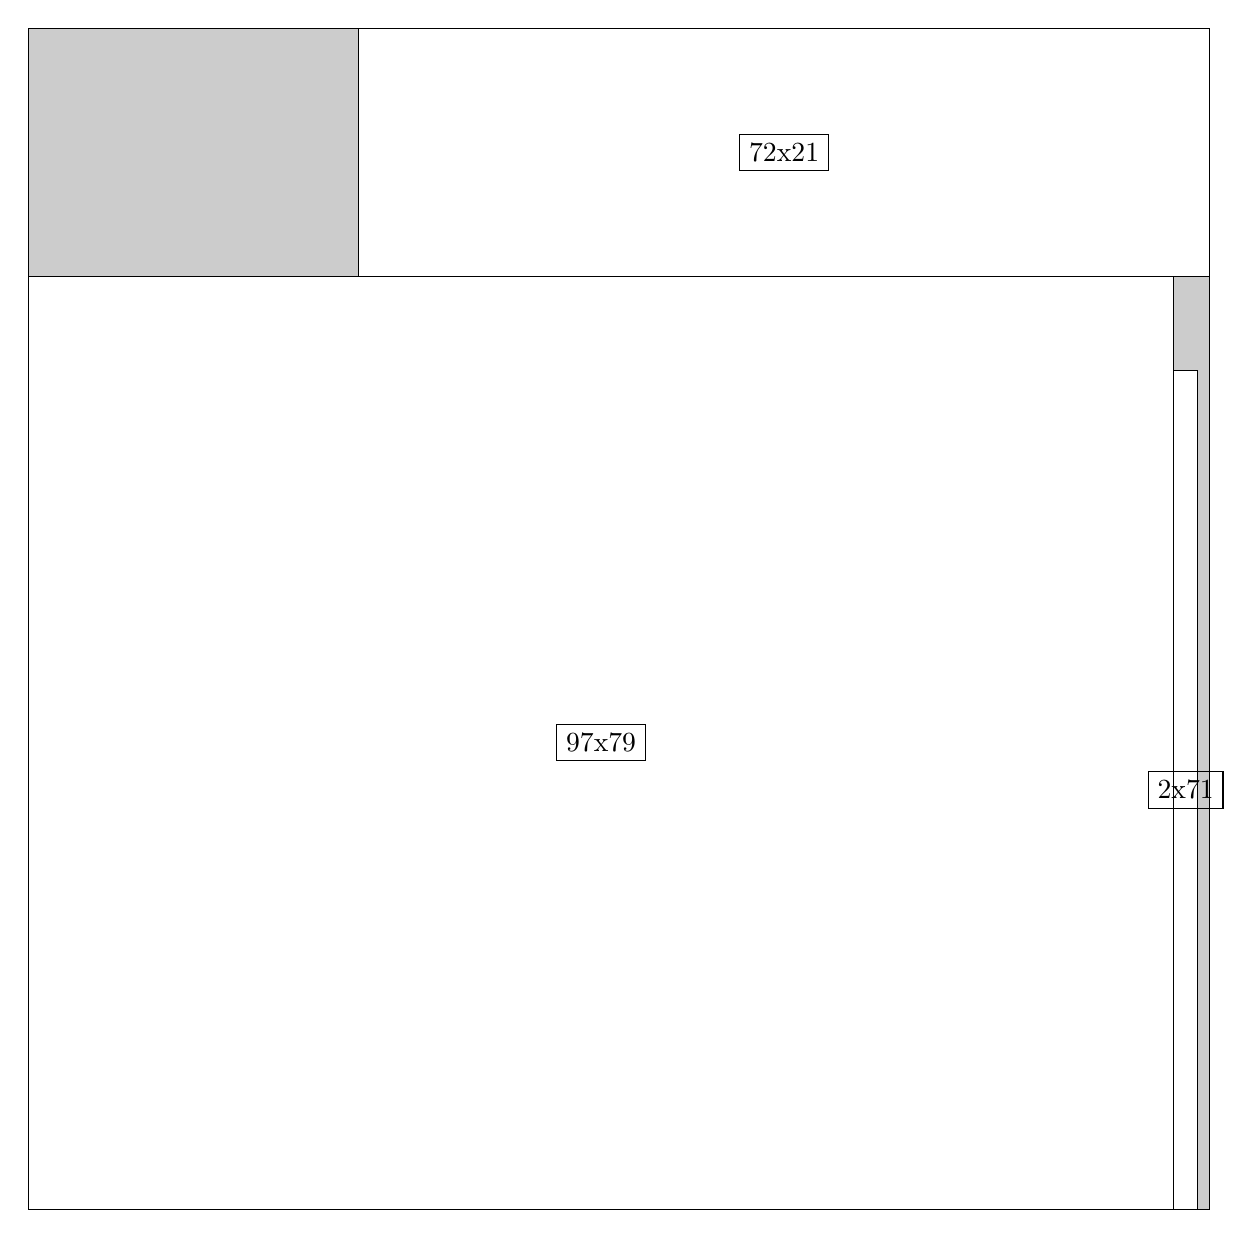
\begin{tikzpicture}[shorten >=1pt,scale=1.0,every node/.style={scale=1.0},->]
\tikzstyle{vertex}=[circle,fill=black!25,minimum size=14pt,inner sep=0pt]
\filldraw[fill=gray!40!white, draw=black] (0,0) rectangle (15.0,15.0);
\foreach \name/\x/\y/\w/\h in {97x79/0.0/0.0/14.549999999999999/11.85,72x21/4.2/11.85/10.799999999999999/3.15,2x71/14.549999999999999/0.0/0.3/10.65}
\filldraw[fill=white!40!white, draw=black] (\x,\y) rectangle node[draw] (\name) {\name} ++(\w,\h);
\end{tikzpicture}


w =97 , h =79 , x =0 , y =0 , v =7663
\par
w =72 , h =21 , x =28 , y =79 , v =1512
\par
w =2 , h =71 , x =97 , y =0 , v =142
\par
\newpage


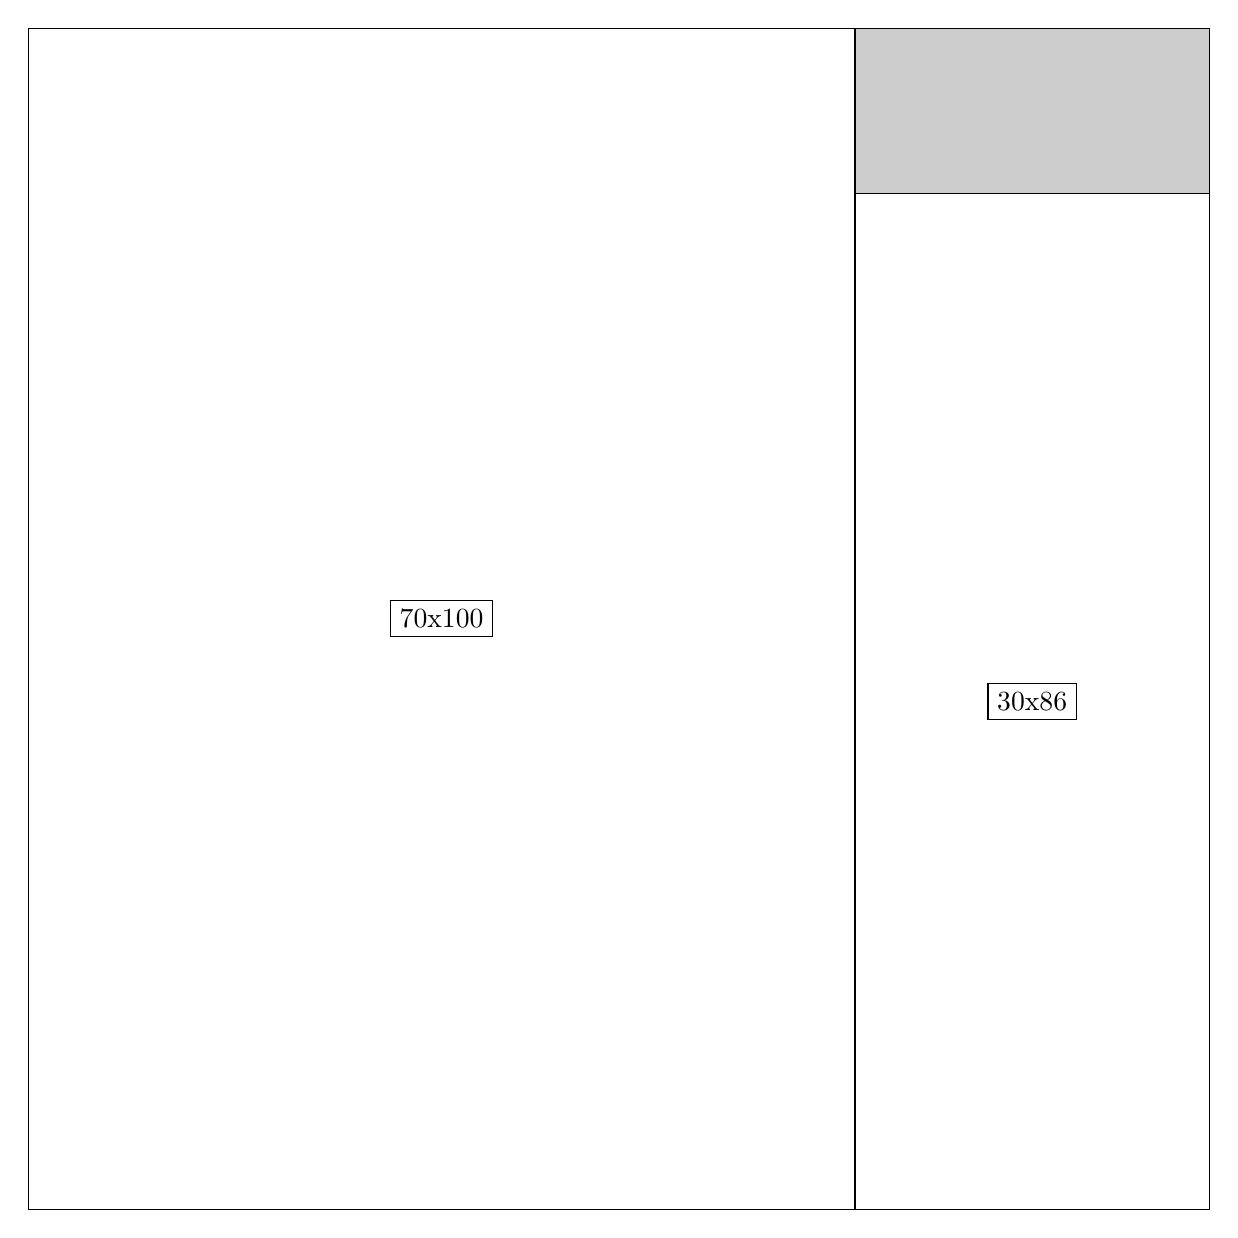
\begin{tikzpicture}[shorten >=1pt,scale=1.0,every node/.style={scale=1.0},->]
\tikzstyle{vertex}=[circle,fill=black!25,minimum size=14pt,inner sep=0pt]
\filldraw[fill=gray!40!white, draw=black] (0,0) rectangle (15.0,15.0);
\foreach \name/\x/\y/\w/\h in {70x100/0.0/0.0/10.5/15.0,30x86/10.5/0.0/4.5/12.9}
\filldraw[fill=white!40!white, draw=black] (\x,\y) rectangle node[draw] (\name) {\name} ++(\w,\h);
\end{tikzpicture}


w =70 , h =100 , x =0 , y =0 , v =7000
\par
w =30 , h =86 , x =70 , y =0 , v =2580
\par
\newpage


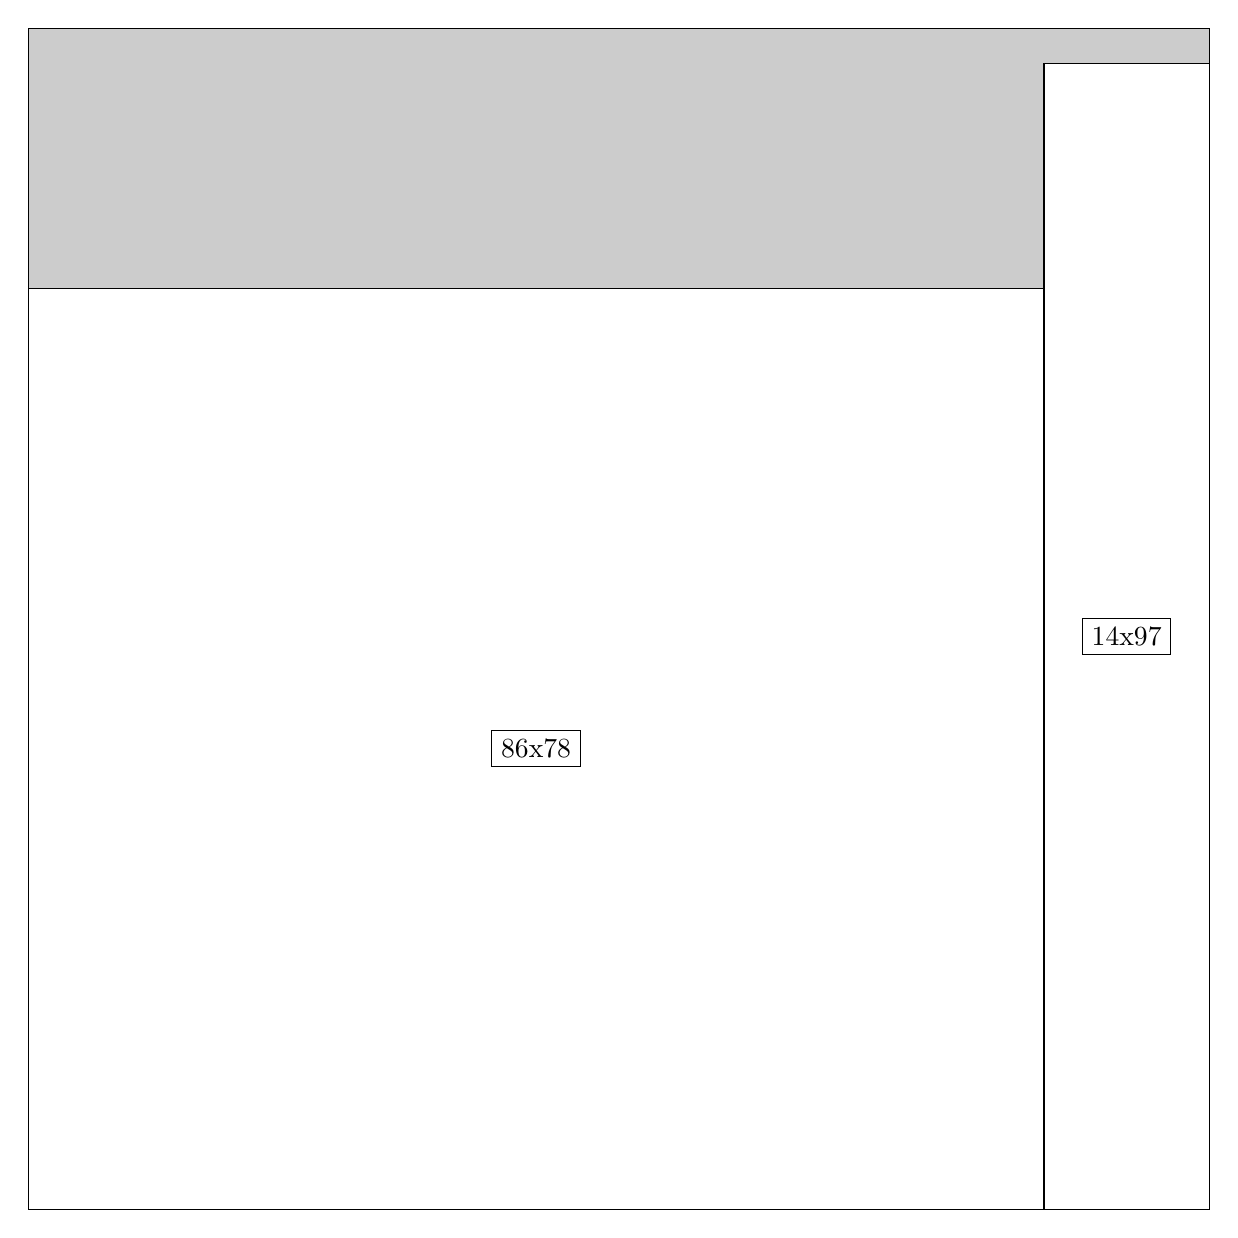
\begin{tikzpicture}[shorten >=1pt,scale=1.0,every node/.style={scale=1.0},->]
\tikzstyle{vertex}=[circle,fill=black!25,minimum size=14pt,inner sep=0pt]
\filldraw[fill=gray!40!white, draw=black] (0,0) rectangle (15.0,15.0);
\foreach \name/\x/\y/\w/\h in {86x78/0.0/0.0/12.9/11.7,14x97/12.9/0.0/2.1/14.549999999999999}
\filldraw[fill=white!40!white, draw=black] (\x,\y) rectangle node[draw] (\name) {\name} ++(\w,\h);
\end{tikzpicture}


w =86 , h =78 , x =0 , y =0 , v =6708
\par
w =14 , h =97 , x =86 , y =0 , v =1358
\par
\newpage


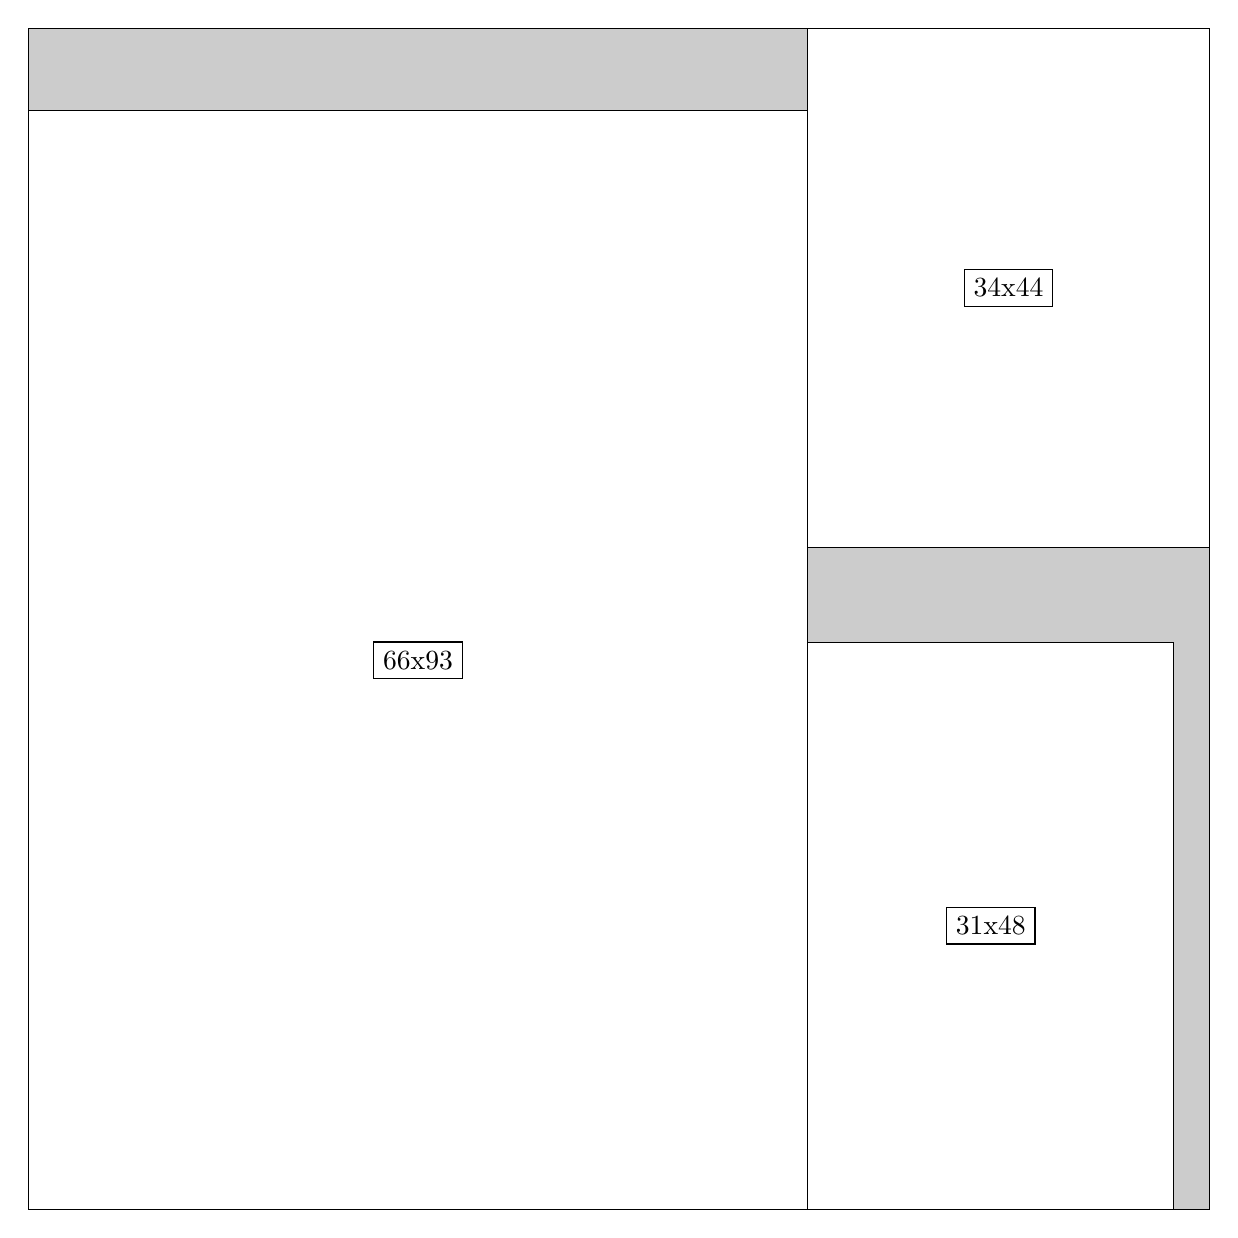
\begin{tikzpicture}[shorten >=1pt,scale=1.0,every node/.style={scale=1.0},->]
\tikzstyle{vertex}=[circle,fill=black!25,minimum size=14pt,inner sep=0pt]
\filldraw[fill=gray!40!white, draw=black] (0,0) rectangle (15.0,15.0);
\foreach \name/\x/\y/\w/\h in {66x93/0.0/0.0/9.9/13.95,34x44/9.9/8.4/5.1/6.6,31x48/9.9/0.0/4.6499999999999995/7.199999999999999}
\filldraw[fill=white!40!white, draw=black] (\x,\y) rectangle node[draw] (\name) {\name} ++(\w,\h);
\end{tikzpicture}


w =66 , h =93 , x =0 , y =0 , v =6138
\par
w =34 , h =44 , x =66 , y =56 , v =1496
\par
w =31 , h =48 , x =66 , y =0 , v =1488
\par
\newpage


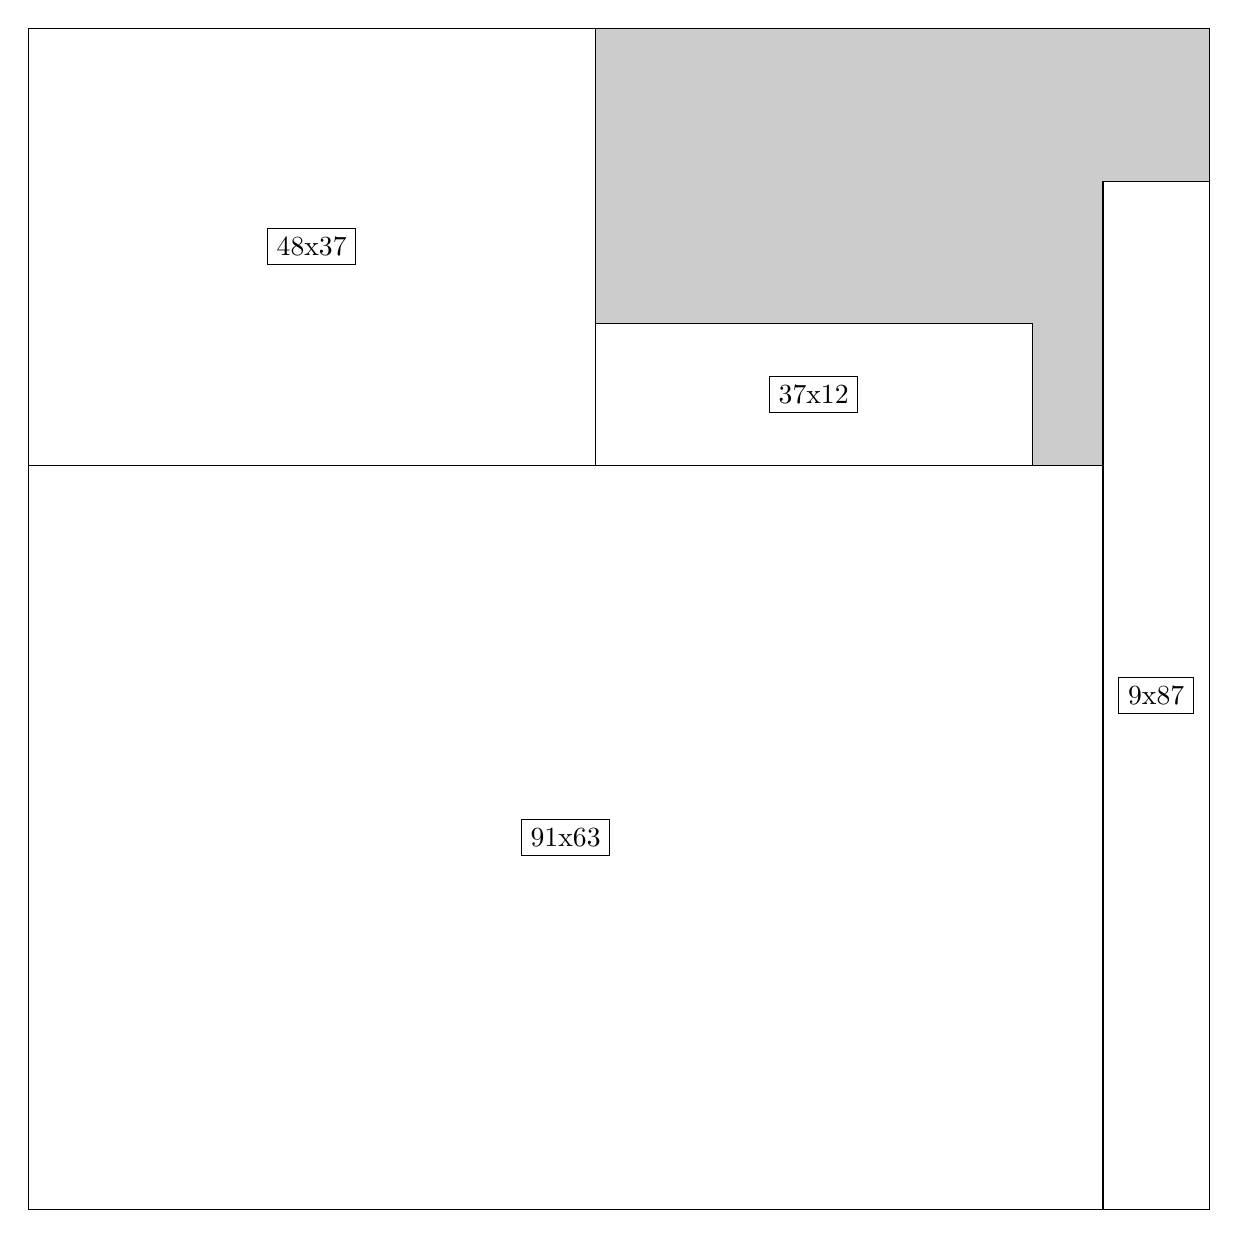
\begin{tikzpicture}[shorten >=1pt,scale=1.0,every node/.style={scale=1.0},->]
\tikzstyle{vertex}=[circle,fill=black!25,minimum size=14pt,inner sep=0pt]
\filldraw[fill=gray!40!white, draw=black] (0,0) rectangle (15.0,15.0);
\foreach \name/\x/\y/\w/\h in {91x63/0.0/0.0/13.65/9.45,48x37/0.0/9.45/7.199999999999999/5.55,9x87/13.65/0.0/1.3499999999999999/13.049999999999999,37x12/7.199999999999999/9.45/5.55/1.7999999999999998}
\filldraw[fill=white!40!white, draw=black] (\x,\y) rectangle node[draw] (\name) {\name} ++(\w,\h);
\end{tikzpicture}


w =91 , h =63 , x =0 , y =0 , v =5733
\par
w =48 , h =37 , x =0 , y =63 , v =1776
\par
w =9 , h =87 , x =91 , y =0 , v =783
\par
w =37 , h =12 , x =48 , y =63 , v =444
\par
\newpage


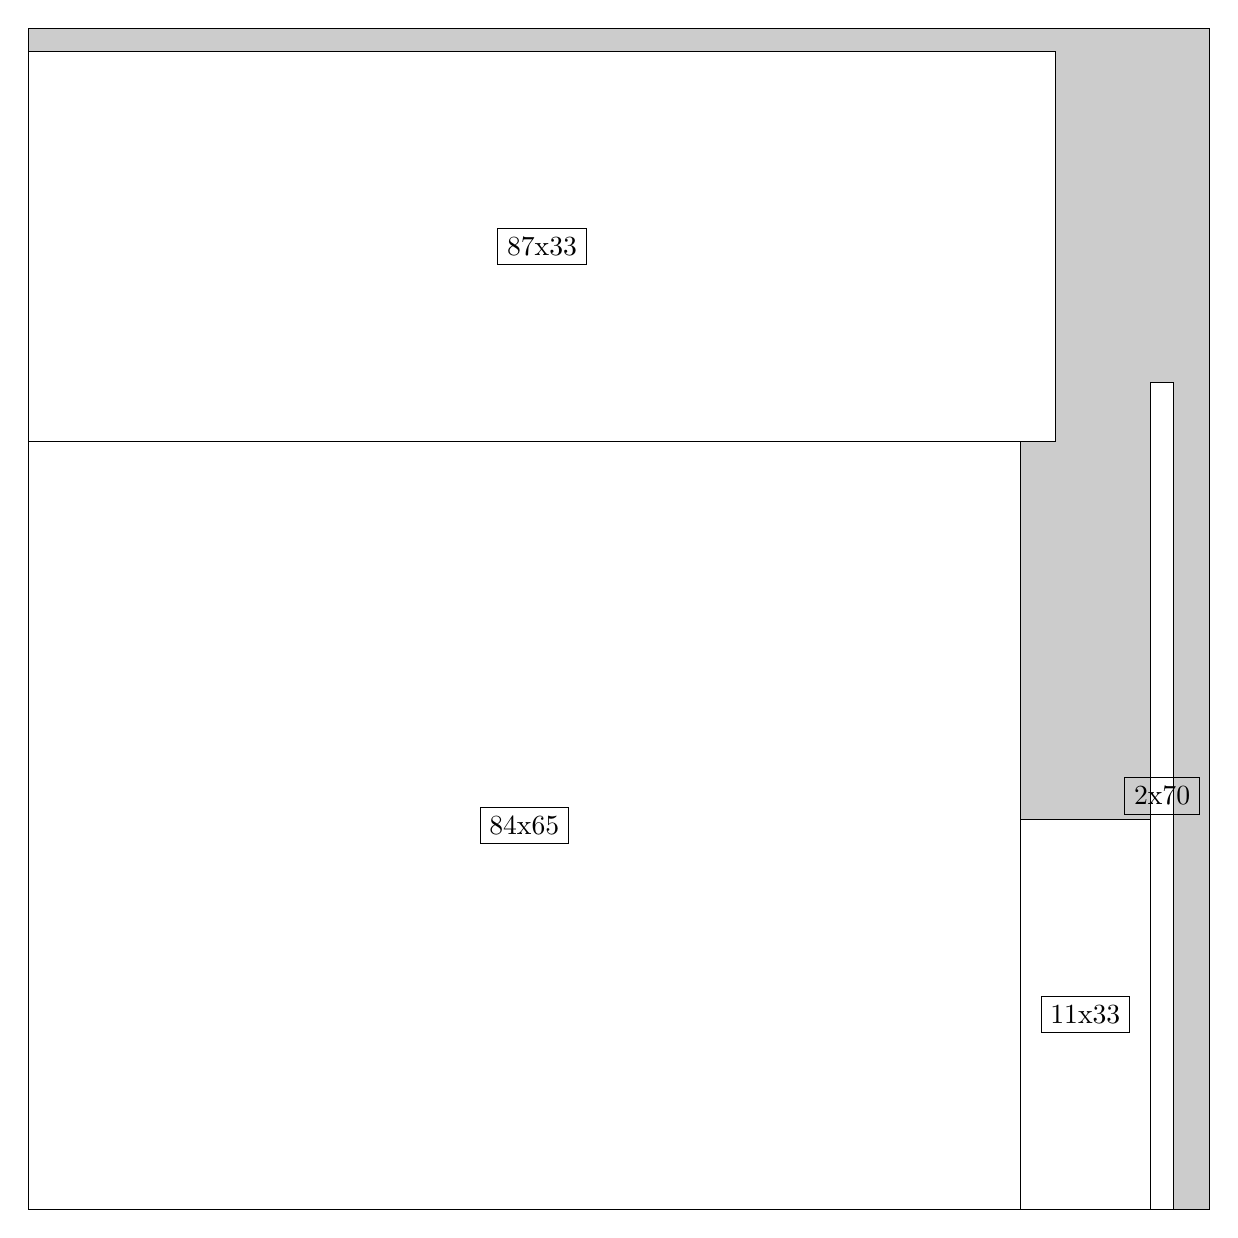
\begin{tikzpicture}[shorten >=1pt,scale=1.0,every node/.style={scale=1.0},->]
\tikzstyle{vertex}=[circle,fill=black!25,minimum size=14pt,inner sep=0pt]
\filldraw[fill=gray!40!white, draw=black] (0,0) rectangle (15.0,15.0);
\foreach \name/\x/\y/\w/\h in {84x65/0.0/0.0/12.6/9.75,87x33/0.0/9.75/13.049999999999999/4.95,11x33/12.6/0.0/1.65/4.95,2x70/14.25/0.0/0.3/10.5}
\filldraw[fill=white!40!white, draw=black] (\x,\y) rectangle node[draw] (\name) {\name} ++(\w,\h);
\end{tikzpicture}


w =84 , h =65 , x =0 , y =0 , v =5460
\par
w =87 , h =33 , x =0 , y =65 , v =2871
\par
w =11 , h =33 , x =84 , y =0 , v =363
\par
w =2 , h =70 , x =95 , y =0 , v =140
\par
\newpage


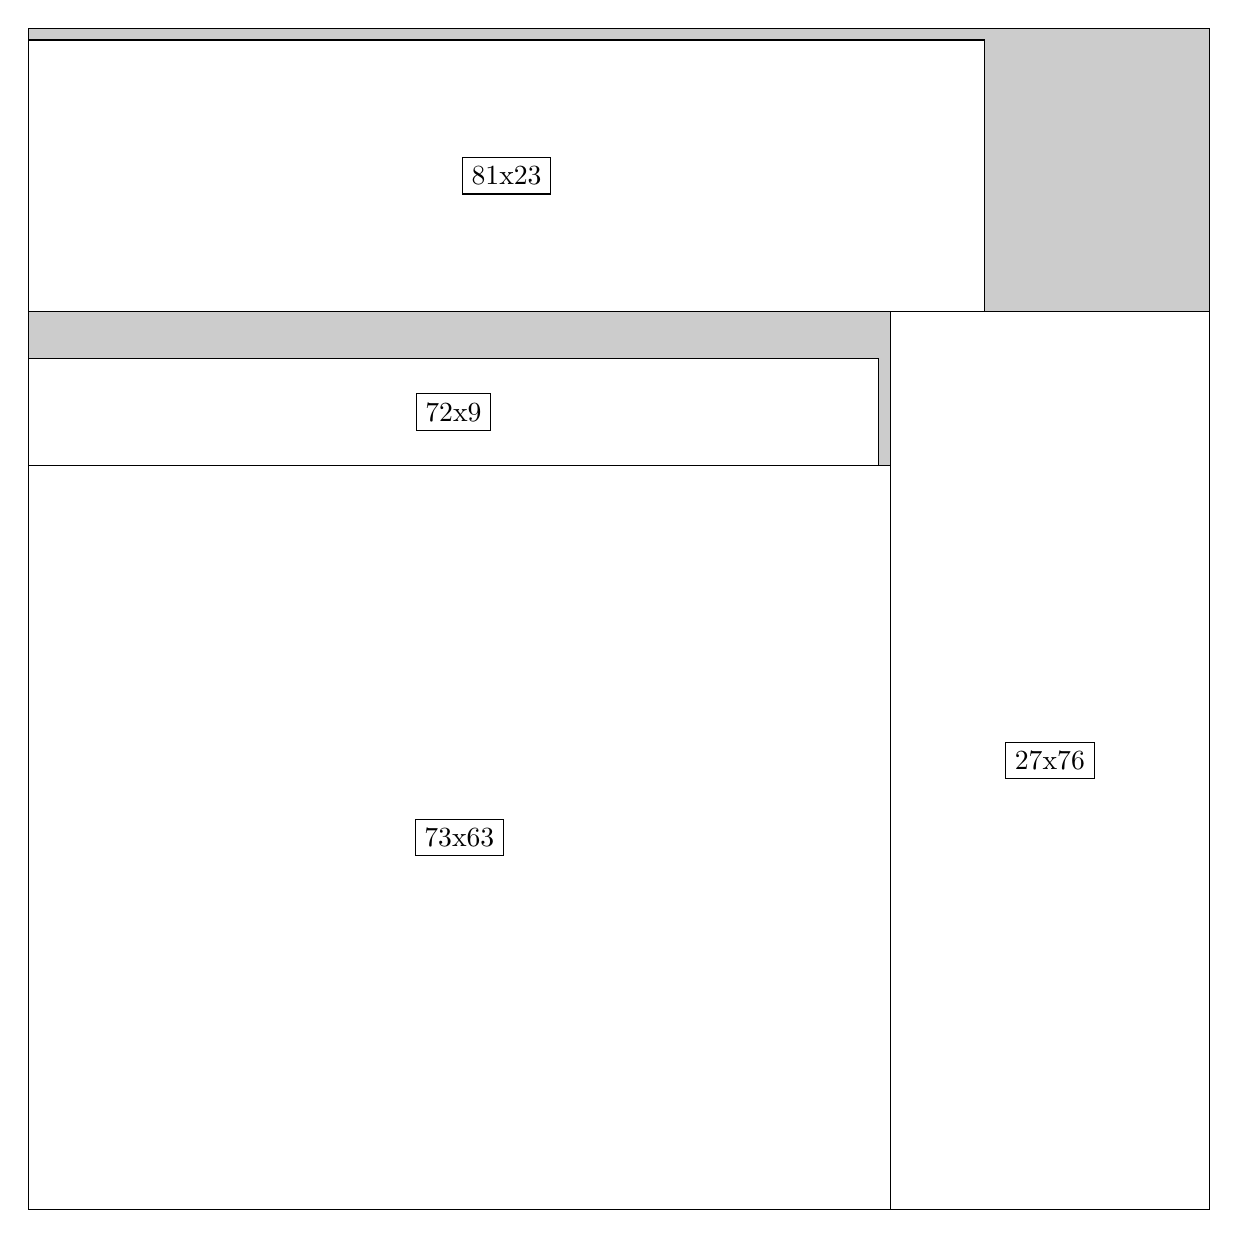
\begin{tikzpicture}[shorten >=1pt,scale=1.0,every node/.style={scale=1.0},->]
\tikzstyle{vertex}=[circle,fill=black!25,minimum size=14pt,inner sep=0pt]
\filldraw[fill=gray!40!white, draw=black] (0,0) rectangle (15.0,15.0);
\foreach \name/\x/\y/\w/\h in {73x63/0.0/0.0/10.95/9.45,27x76/10.95/0.0/4.05/11.4,81x23/0.0/11.4/12.15/3.4499999999999997,72x9/0.0/9.45/10.799999999999999/1.3499999999999999}
\filldraw[fill=white!40!white, draw=black] (\x,\y) rectangle node[draw] (\name) {\name} ++(\w,\h);
\end{tikzpicture}


w =73 , h =63 , x =0 , y =0 , v =4599
\par
w =27 , h =76 , x =73 , y =0 , v =2052
\par
w =81 , h =23 , x =0 , y =76 , v =1863
\par
w =72 , h =9 , x =0 , y =63 , v =648
\par
\newpage


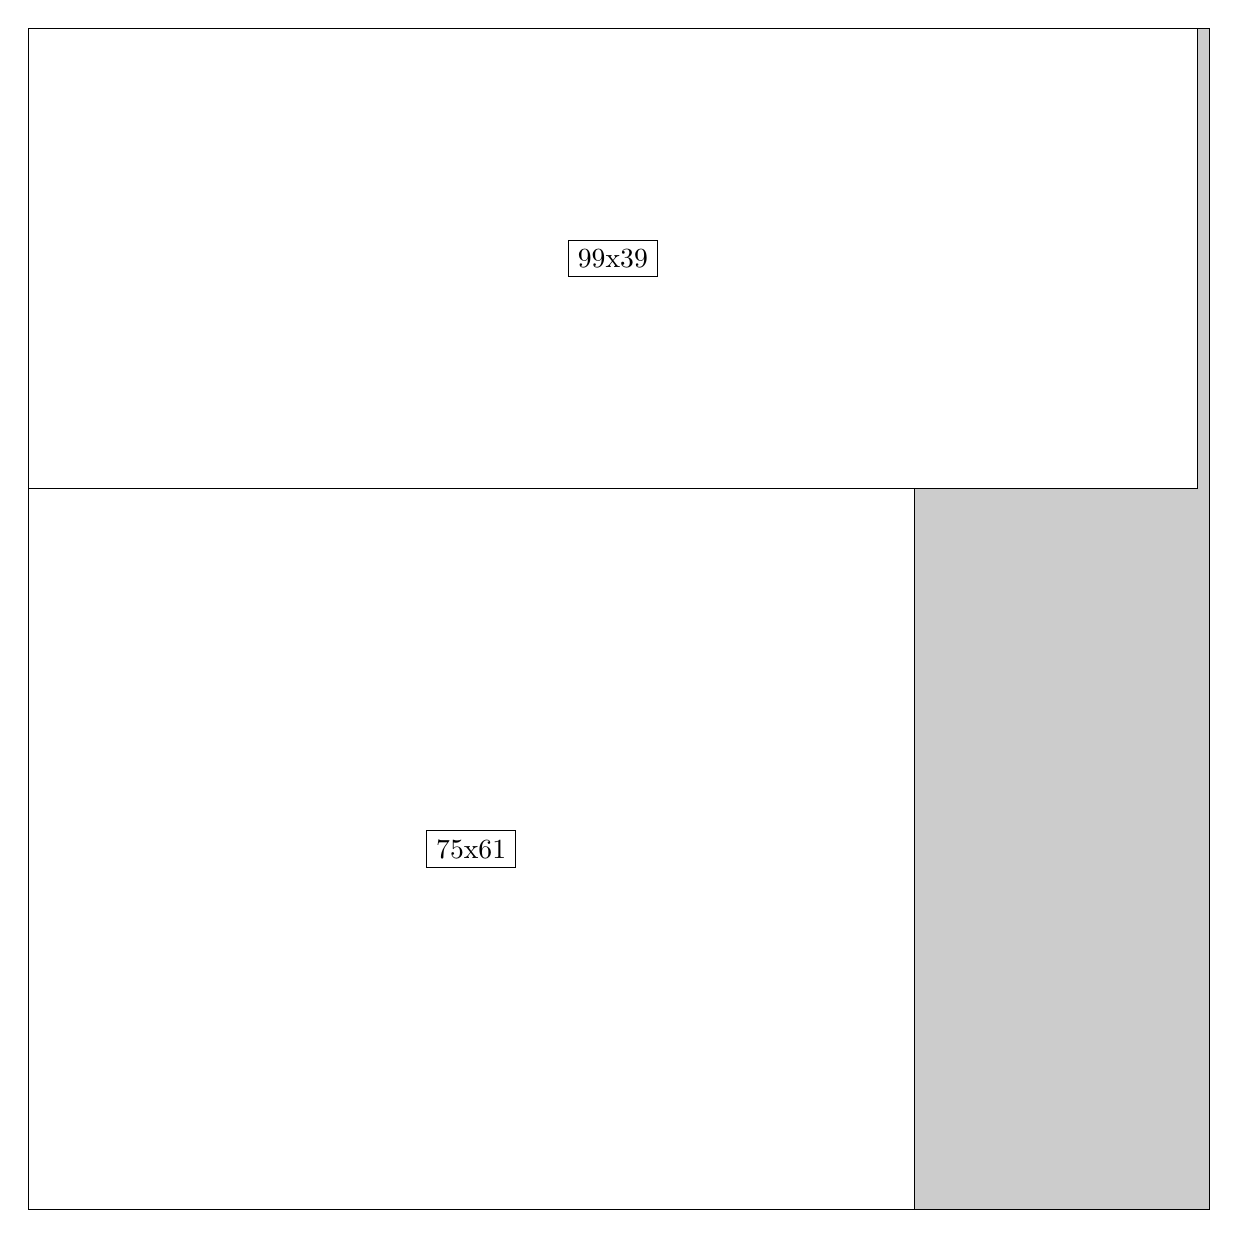
\begin{tikzpicture}[shorten >=1pt,scale=1.0,every node/.style={scale=1.0},->]
\tikzstyle{vertex}=[circle,fill=black!25,minimum size=14pt,inner sep=0pt]
\filldraw[fill=gray!40!white, draw=black] (0,0) rectangle (15.0,15.0);
\foreach \name/\x/\y/\w/\h in {75x61/0.0/0.0/11.25/9.15,99x39/0.0/9.15/14.85/5.85}
\filldraw[fill=white!40!white, draw=black] (\x,\y) rectangle node[draw] (\name) {\name} ++(\w,\h);
\end{tikzpicture}


w =75 , h =61 , x =0 , y =0 , v =4575
\par
w =99 , h =39 , x =0 , y =61 , v =3861
\par
\newpage


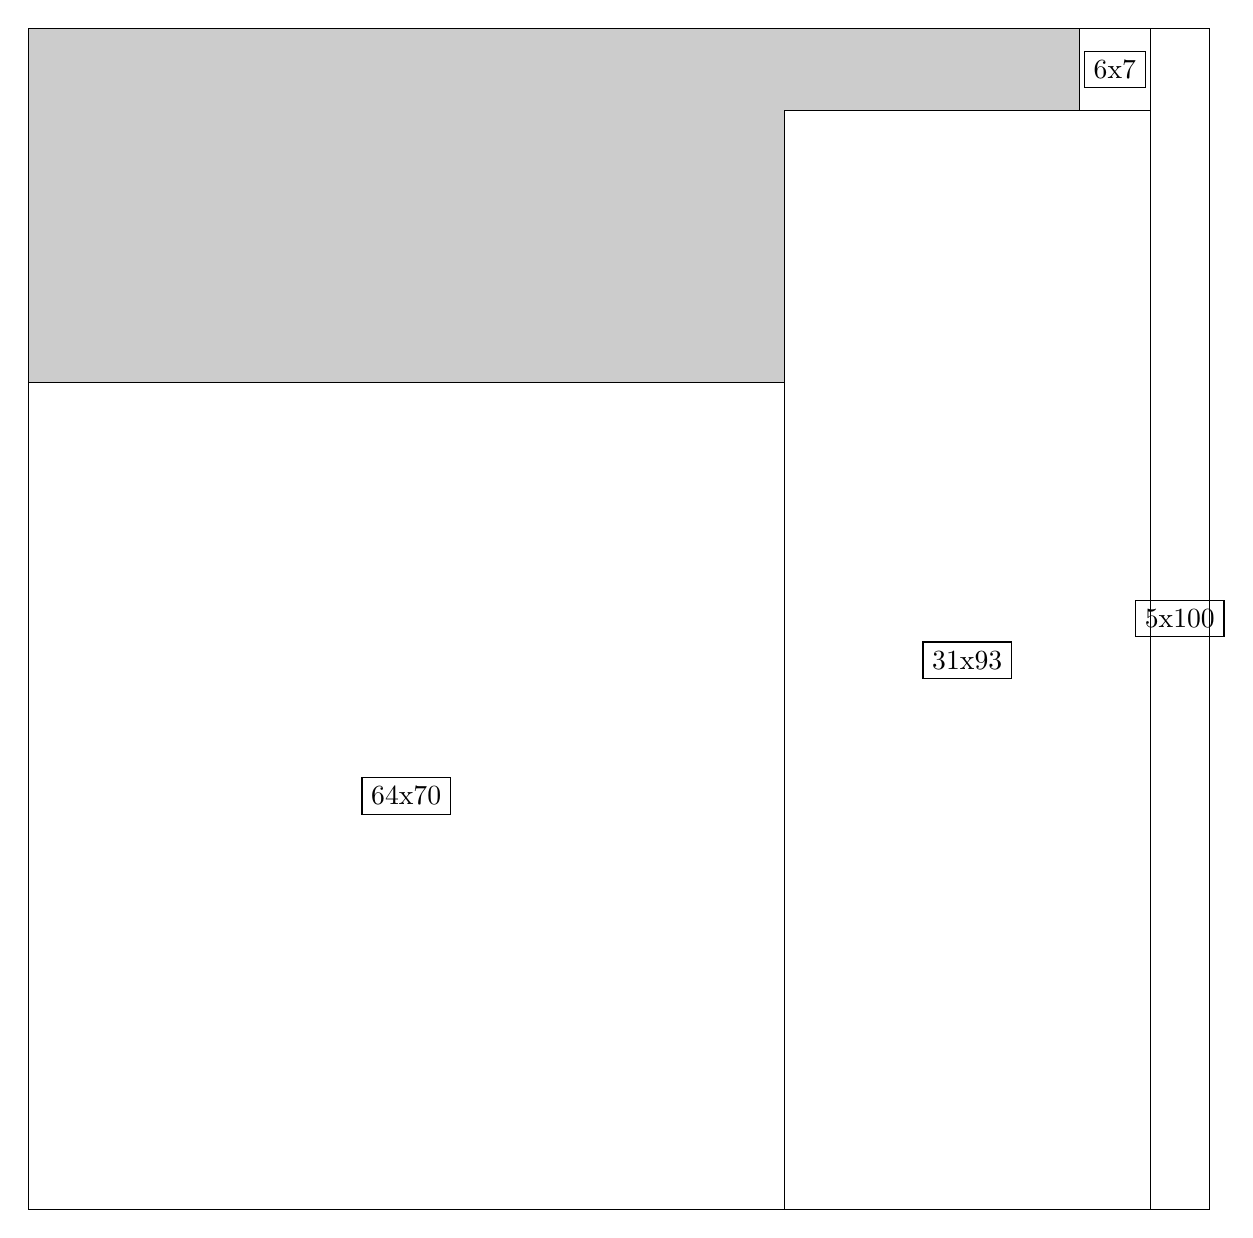
\begin{tikzpicture}[shorten >=1pt,scale=1.0,every node/.style={scale=1.0},->]
\tikzstyle{vertex}=[circle,fill=black!25,minimum size=14pt,inner sep=0pt]
\filldraw[fill=gray!40!white, draw=black] (0,0) rectangle (15.0,15.0);
\foreach \name/\x/\y/\w/\h in {64x70/0.0/0.0/9.6/10.5,31x93/9.6/0.0/4.6499999999999995/13.95,5x100/14.25/0.0/0.75/15.0,6x7/13.35/13.95/0.8999999999999999/1.05}
\filldraw[fill=white!40!white, draw=black] (\x,\y) rectangle node[draw] (\name) {\name} ++(\w,\h);
\end{tikzpicture}


w =64 , h =70 , x =0 , y =0 , v =4480
\par
w =31 , h =93 , x =64 , y =0 , v =2883
\par
w =5 , h =100 , x =95 , y =0 , v =500
\par
w =6 , h =7 , x =89 , y =93 , v =42
\par
\newpage


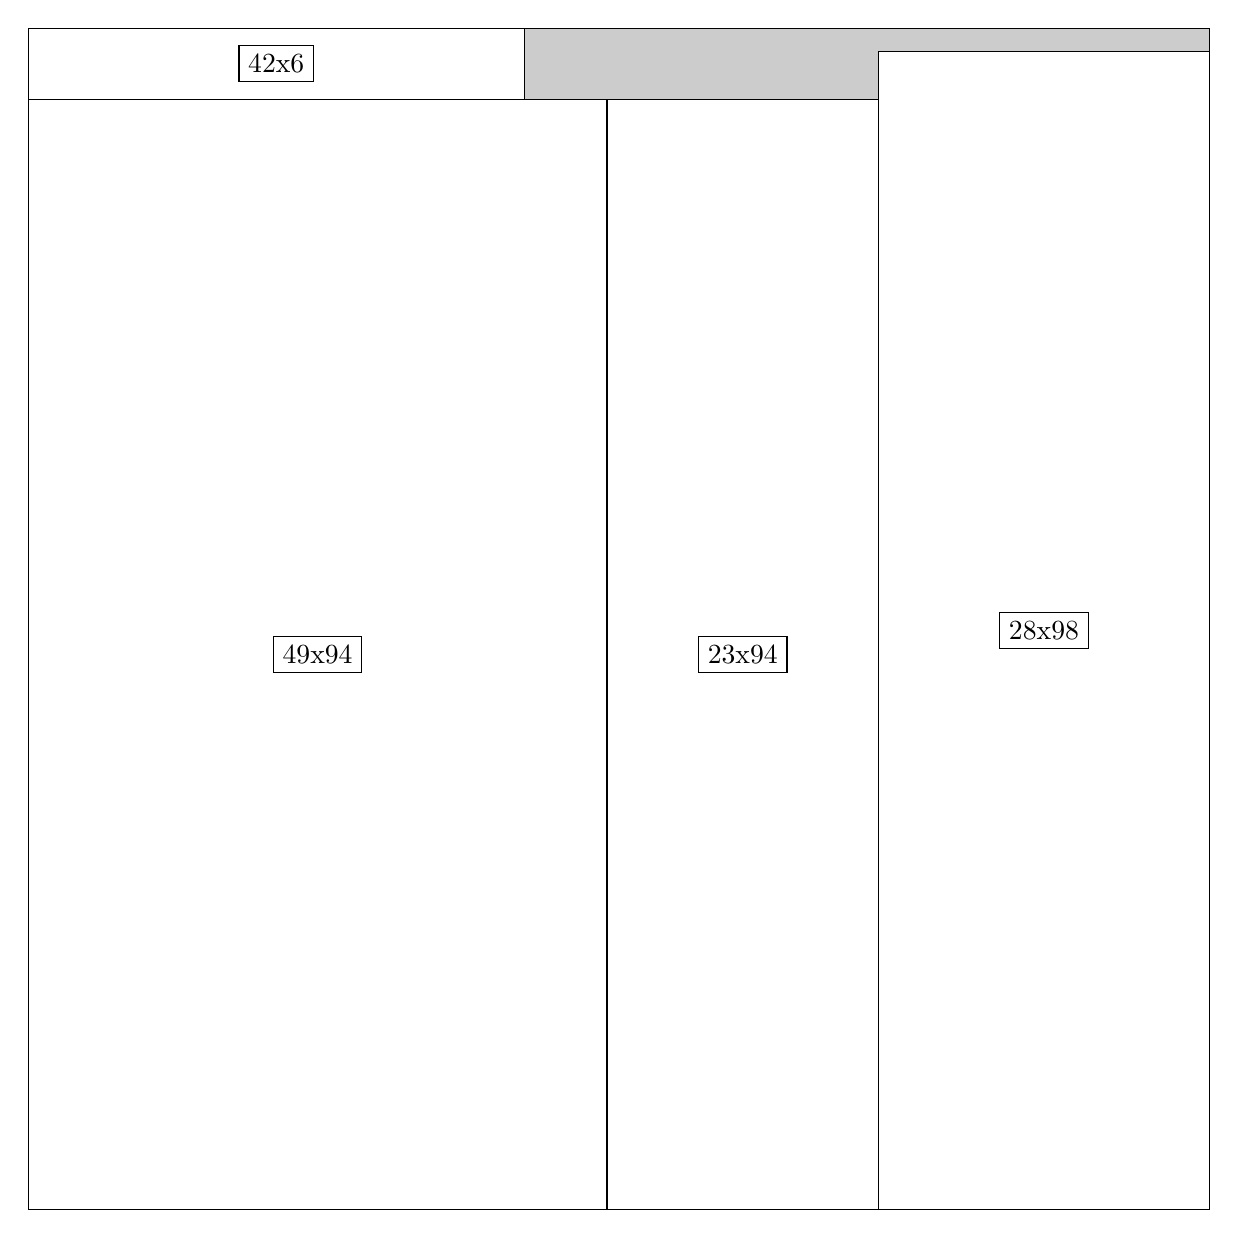
\begin{tikzpicture}[shorten >=1pt,scale=1.0,every node/.style={scale=1.0},->]
\tikzstyle{vertex}=[circle,fill=black!25,minimum size=14pt,inner sep=0pt]
\filldraw[fill=gray!40!white, draw=black] (0,0) rectangle (15.0,15.0);
\foreach \name/\x/\y/\w/\h in {49x94/0.0/0.0/7.35/14.1,28x98/10.799999999999999/0.0/4.2/14.7,23x94/7.35/0.0/3.4499999999999997/14.1,42x6/0.0/14.1/6.3/0.8999999999999999}
\filldraw[fill=white!40!white, draw=black] (\x,\y) rectangle node[draw] (\name) {\name} ++(\w,\h);
\end{tikzpicture}


w =49 , h =94 , x =0 , y =0 , v =4606
\par
w =28 , h =98 , x =72 , y =0 , v =2744
\par
w =23 , h =94 , x =49 , y =0 , v =2162
\par
w =42 , h =6 , x =0 , y =94 , v =252
\par
\newpage


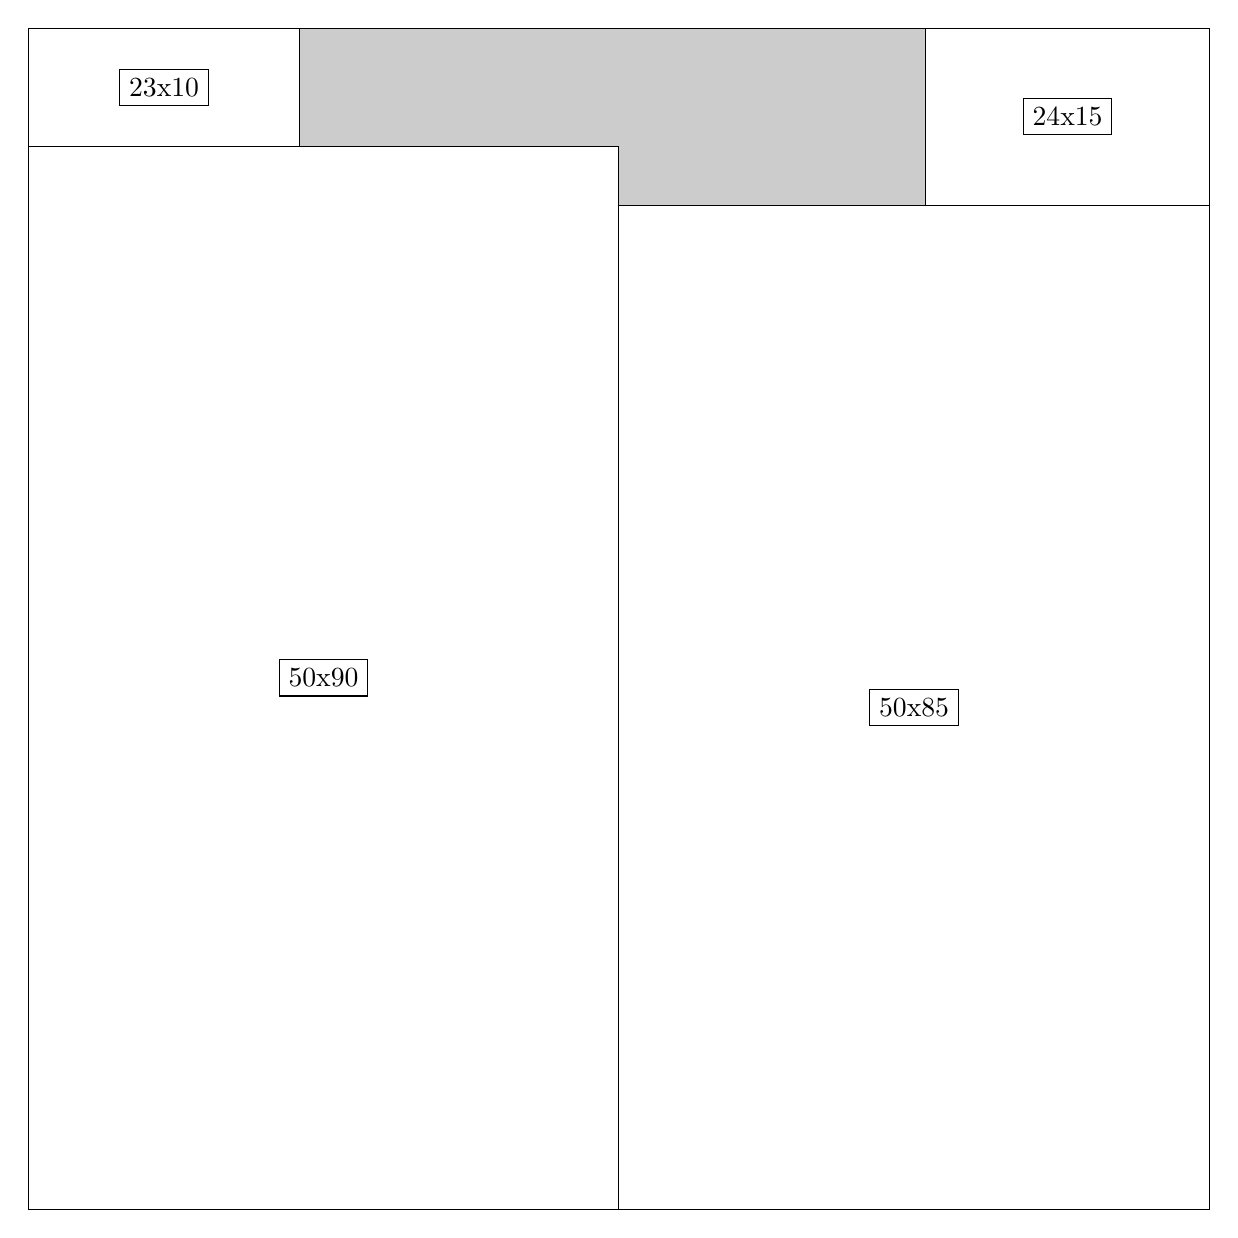
\begin{tikzpicture}[shorten >=1pt,scale=1.0,every node/.style={scale=1.0},->]
\tikzstyle{vertex}=[circle,fill=black!25,minimum size=14pt,inner sep=0pt]
\filldraw[fill=gray!40!white, draw=black] (0,0) rectangle (15.0,15.0);
\foreach \name/\x/\y/\w/\h in {50x90/0.0/0.0/7.5/13.5,50x85/7.5/0.0/7.5/12.75,24x15/11.4/12.75/3.5999999999999996/2.25,23x10/0.0/13.5/3.4499999999999997/1.5}
\filldraw[fill=white!40!white, draw=black] (\x,\y) rectangle node[draw] (\name) {\name} ++(\w,\h);
\end{tikzpicture}


w =50 , h =90 , x =0 , y =0 , v =4500
\par
w =50 , h =85 , x =50 , y =0 , v =4250
\par
w =24 , h =15 , x =76 , y =85 , v =360
\par
w =23 , h =10 , x =0 , y =90 , v =230
\par
\newpage


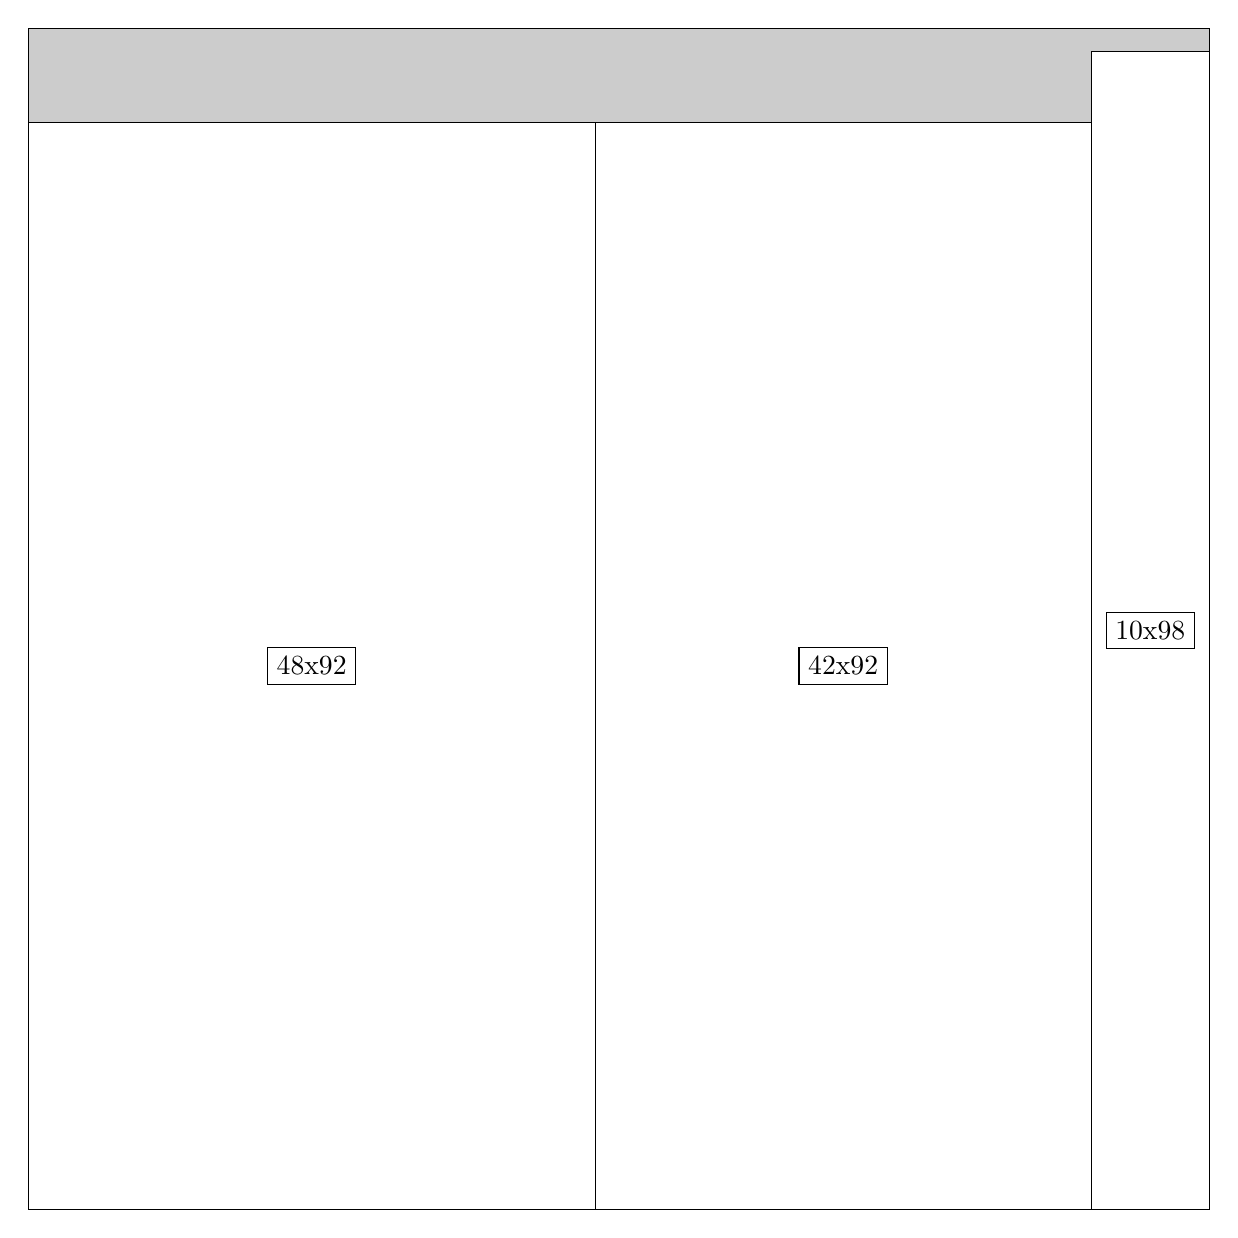
\begin{tikzpicture}[shorten >=1pt,scale=1.0,every node/.style={scale=1.0},->]
\tikzstyle{vertex}=[circle,fill=black!25,minimum size=14pt,inner sep=0pt]
\filldraw[fill=gray!40!white, draw=black] (0,0) rectangle (15.0,15.0);
\foreach \name/\x/\y/\w/\h in {48x92/0.0/0.0/7.199999999999999/13.799999999999999,42x92/7.199999999999999/0.0/6.3/13.799999999999999,10x98/13.5/0.0/1.5/14.7}
\filldraw[fill=white!40!white, draw=black] (\x,\y) rectangle node[draw] (\name) {\name} ++(\w,\h);
\end{tikzpicture}


w =48 , h =92 , x =0 , y =0 , v =4416
\par
w =42 , h =92 , x =48 , y =0 , v =3864
\par
w =10 , h =98 , x =90 , y =0 , v =980
\par
\newpage


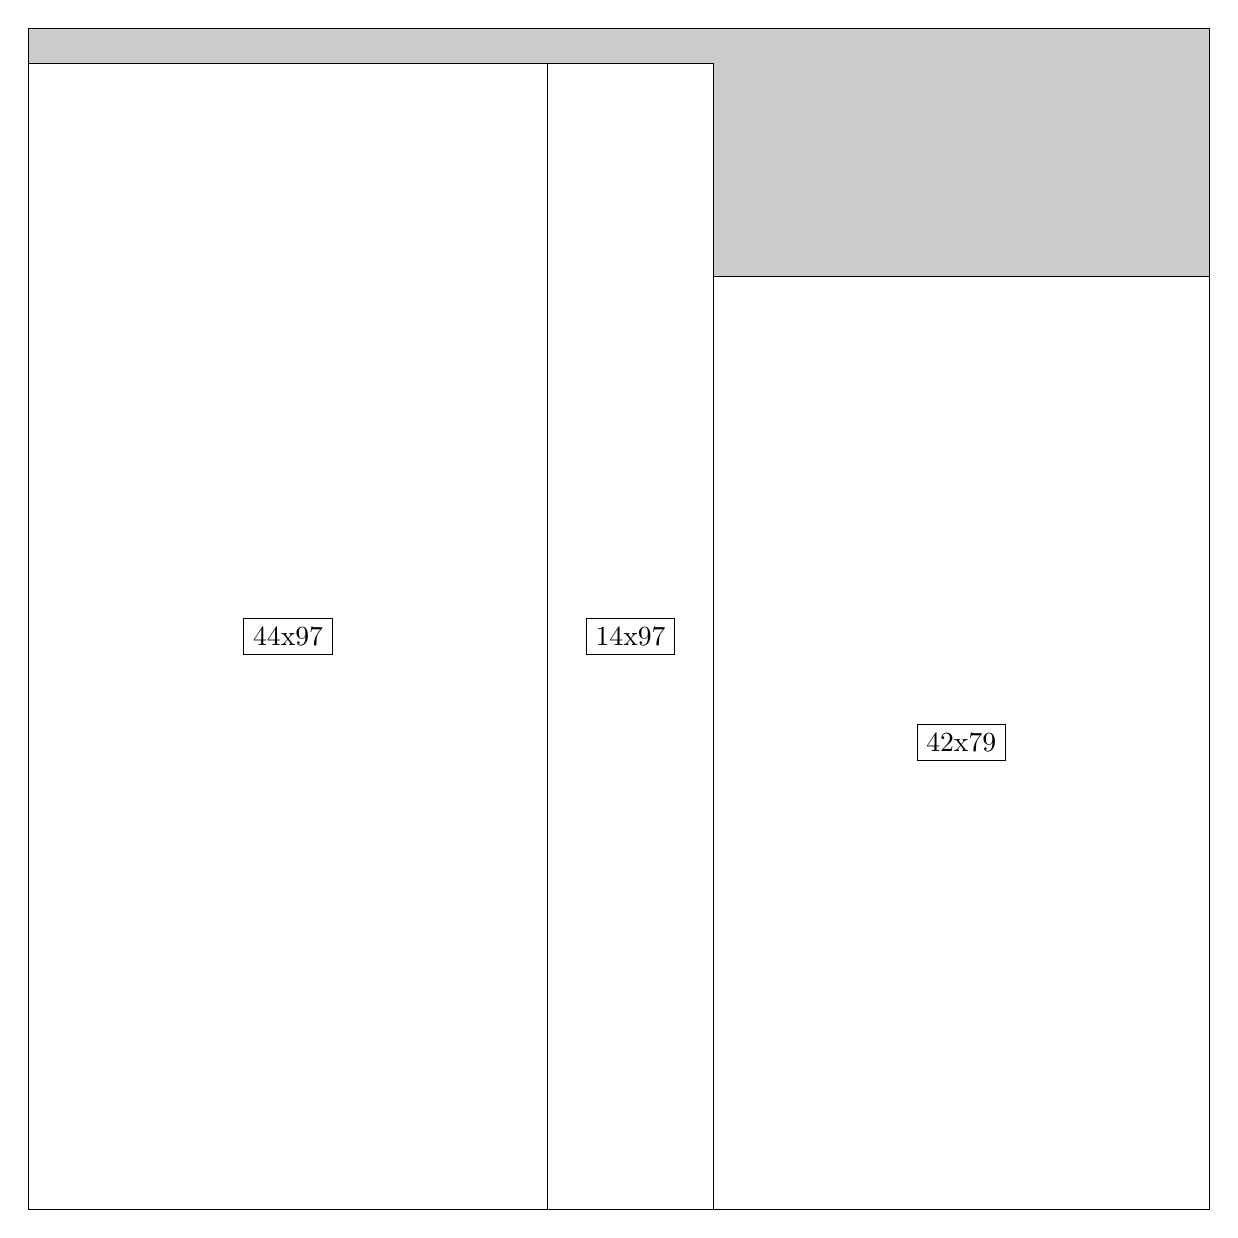
\begin{tikzpicture}[shorten >=1pt,scale=1.0,every node/.style={scale=1.0},->]
\tikzstyle{vertex}=[circle,fill=black!25,minimum size=14pt,inner sep=0pt]
\filldraw[fill=gray!40!white, draw=black] (0,0) rectangle (15.0,15.0);
\foreach \name/\x/\y/\w/\h in {44x97/0.0/0.0/6.6/14.549999999999999,42x79/8.7/0.0/6.3/11.85,14x97/6.6/0.0/2.1/14.549999999999999}
\filldraw[fill=white!40!white, draw=black] (\x,\y) rectangle node[draw] (\name) {\name} ++(\w,\h);
\end{tikzpicture}


w =44 , h =97 , x =0 , y =0 , v =4268
\par
w =42 , h =79 , x =58 , y =0 , v =3318
\par
w =14 , h =97 , x =44 , y =0 , v =1358
\par
\newpage


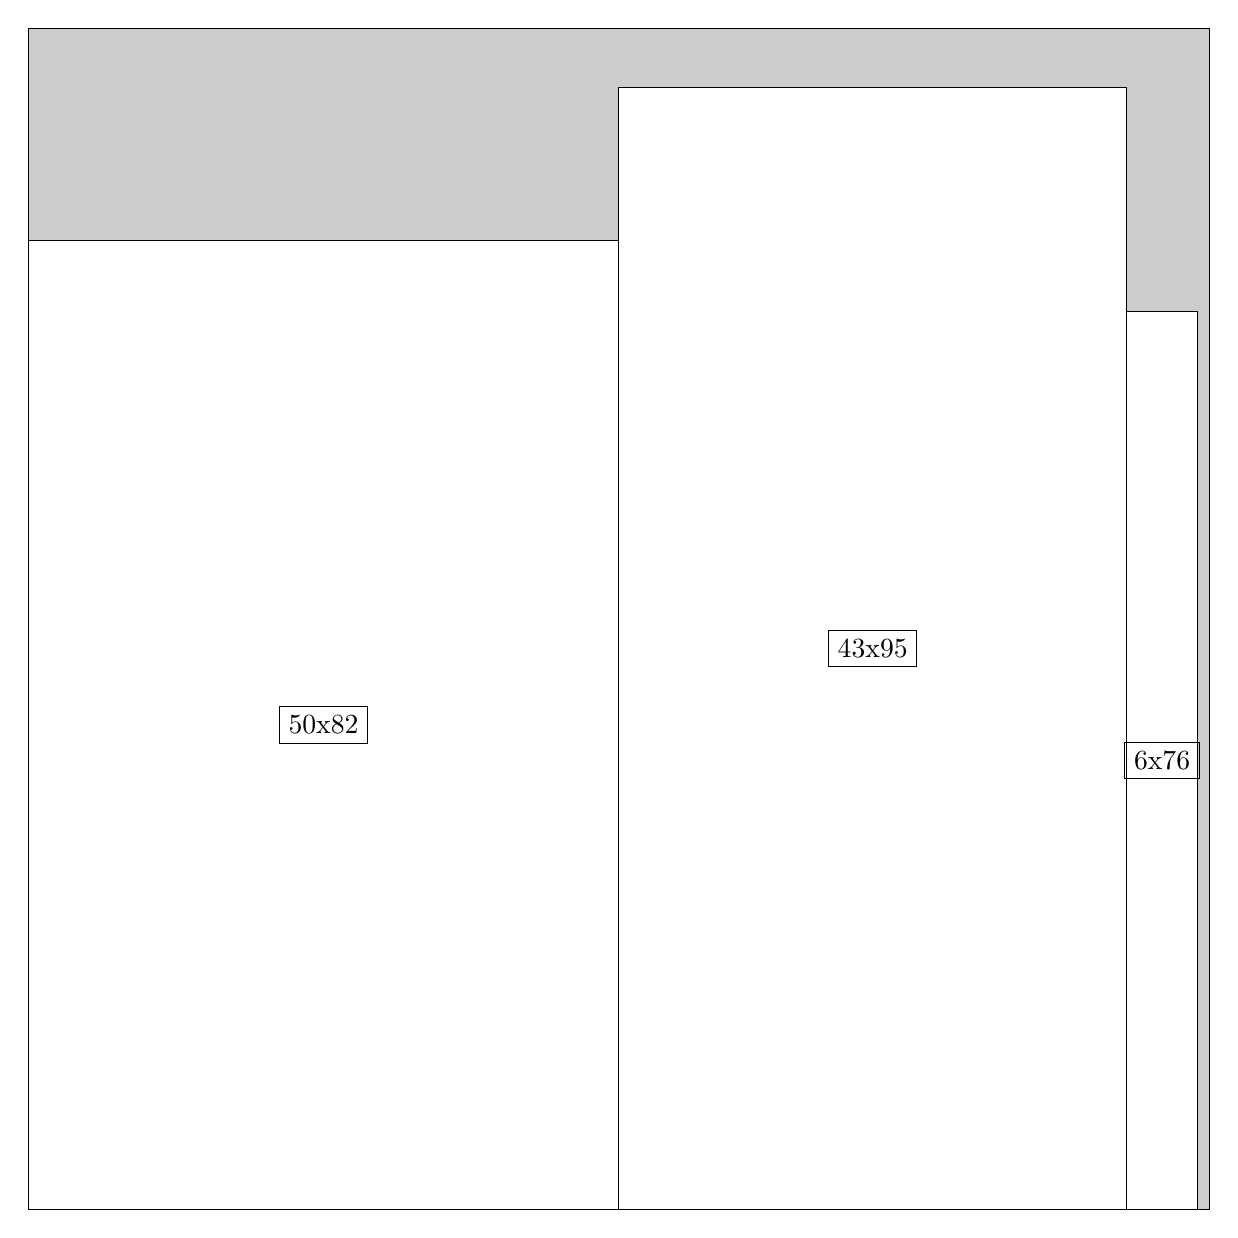
\begin{tikzpicture}[shorten >=1pt,scale=1.0,every node/.style={scale=1.0},->]
\tikzstyle{vertex}=[circle,fill=black!25,minimum size=14pt,inner sep=0pt]
\filldraw[fill=gray!40!white, draw=black] (0,0) rectangle (15.0,15.0);
\foreach \name/\x/\y/\w/\h in {50x82/0.0/0.0/7.5/12.299999999999999,43x95/7.5/0.0/6.45/14.25,6x76/13.95/0.0/0.8999999999999999/11.4}
\filldraw[fill=white!40!white, draw=black] (\x,\y) rectangle node[draw] (\name) {\name} ++(\w,\h);
\end{tikzpicture}


w =50 , h =82 , x =0 , y =0 , v =4100
\par
w =43 , h =95 , x =50 , y =0 , v =4085
\par
w =6 , h =76 , x =93 , y =0 , v =456
\par
\newpage


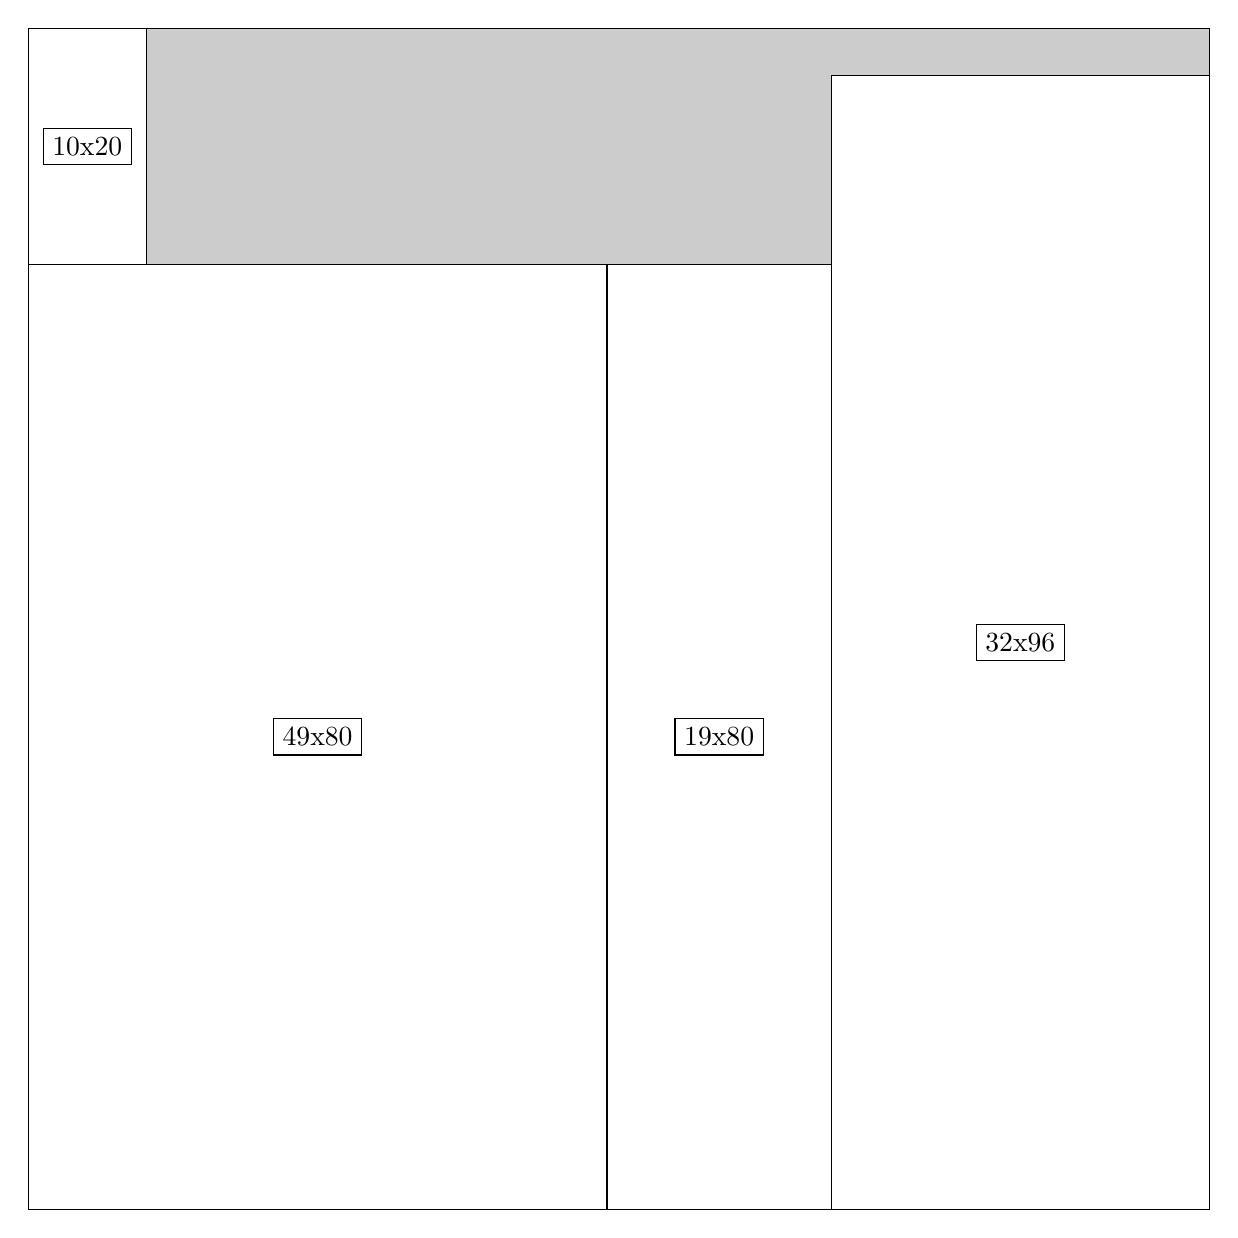
\begin{tikzpicture}[shorten >=1pt,scale=1.0,every node/.style={scale=1.0},->]
\tikzstyle{vertex}=[circle,fill=black!25,minimum size=14pt,inner sep=0pt]
\filldraw[fill=gray!40!white, draw=black] (0,0) rectangle (15.0,15.0);
\foreach \name/\x/\y/\w/\h in {49x80/0.0/0.0/7.35/12.0,32x96/10.2/0.0/4.8/14.399999999999999,19x80/7.35/0.0/2.85/12.0,10x20/0.0/12.0/1.5/3.0}
\filldraw[fill=white!40!white, draw=black] (\x,\y) rectangle node[draw] (\name) {\name} ++(\w,\h);
\end{tikzpicture}


w =49 , h =80 , x =0 , y =0 , v =3920
\par
w =32 , h =96 , x =68 , y =0 , v =3072
\par
w =19 , h =80 , x =49 , y =0 , v =1520
\par
w =10 , h =20 , x =0 , y =80 , v =200
\par
\newpage


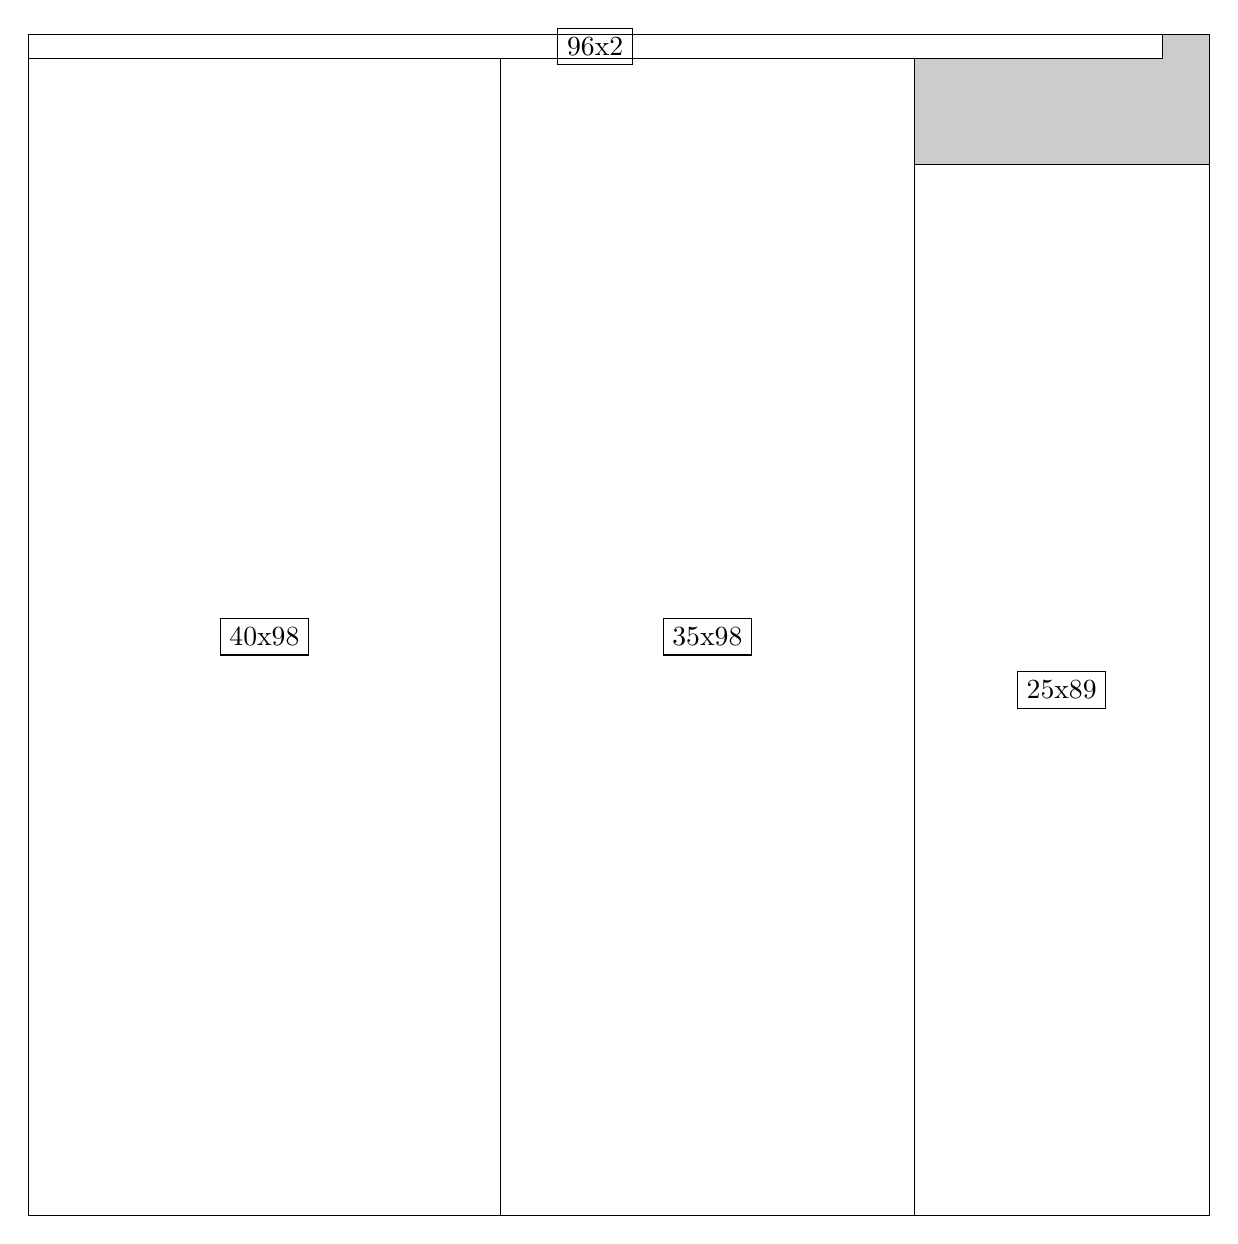
\begin{tikzpicture}[shorten >=1pt,scale=1.0,every node/.style={scale=1.0},->]
\tikzstyle{vertex}=[circle,fill=black!25,minimum size=14pt,inner sep=0pt]
\filldraw[fill=gray!40!white, draw=black] (0,0) rectangle (15.0,15.0);
\foreach \name/\x/\y/\w/\h in {40x98/0.0/0.0/6.0/14.7,35x98/6.0/0.0/5.25/14.7,25x89/11.25/0.0/3.75/13.35,96x2/0.0/14.7/14.399999999999999/0.3}
\filldraw[fill=white!40!white, draw=black] (\x,\y) rectangle node[draw] (\name) {\name} ++(\w,\h);
\end{tikzpicture}


w =40 , h =98 , x =0 , y =0 , v =3920
\par
w =35 , h =98 , x =40 , y =0 , v =3430
\par
w =25 , h =89 , x =75 , y =0 , v =2225
\par
w =96 , h =2 , x =0 , y =98 , v =192
\par
\newpage


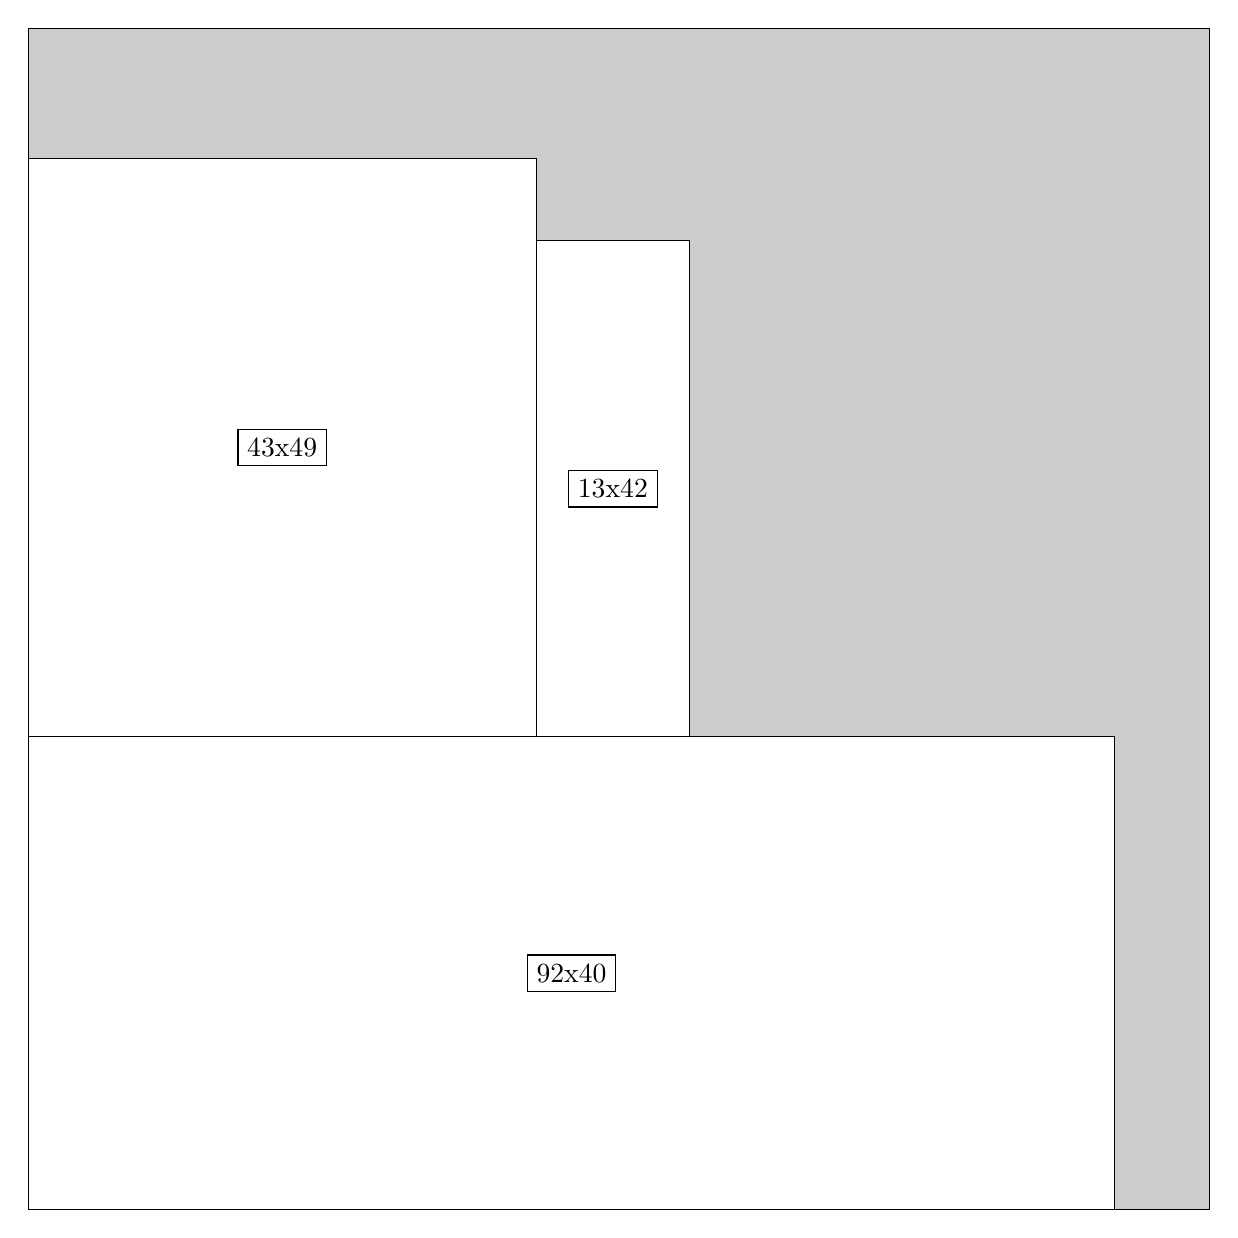
\begin{tikzpicture}[shorten >=1pt,scale=1.0,every node/.style={scale=1.0},->]
\tikzstyle{vertex}=[circle,fill=black!25,minimum size=14pt,inner sep=0pt]
\filldraw[fill=gray!40!white, draw=black] (0,0) rectangle (15.0,15.0);
\foreach \name/\x/\y/\w/\h in {92x40/0.0/0.0/13.799999999999999/6.0,43x49/0.0/6.0/6.45/7.35,13x42/6.45/6.0/1.95/6.3}
\filldraw[fill=white!40!white, draw=black] (\x,\y) rectangle node[draw] (\name) {\name} ++(\w,\h);
\end{tikzpicture}


w =92 , h =40 , x =0 , y =0 , v =3680
\par
w =43 , h =49 , x =0 , y =40 , v =2107
\par
w =13 , h =42 , x =43 , y =40 , v =546
\par
\newpage


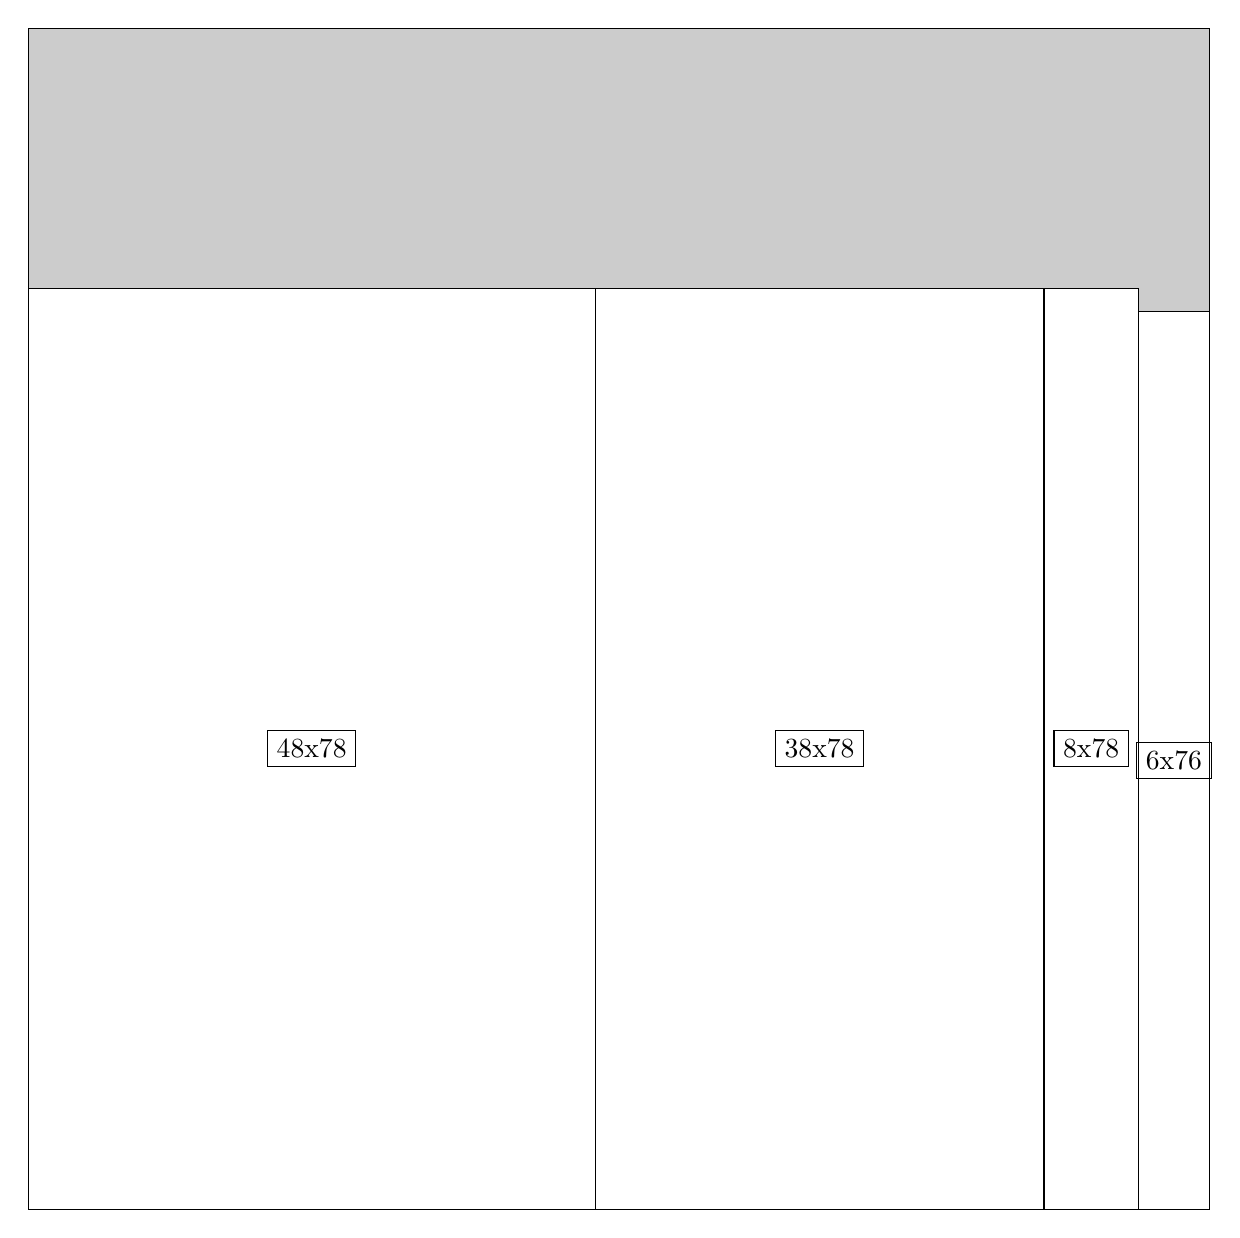
\begin{tikzpicture}[shorten >=1pt,scale=1.0,every node/.style={scale=1.0},->]
\tikzstyle{vertex}=[circle,fill=black!25,minimum size=14pt,inner sep=0pt]
\filldraw[fill=gray!40!white, draw=black] (0,0) rectangle (15.0,15.0);
\foreach \name/\x/\y/\w/\h in {48x78/0.0/0.0/7.199999999999999/11.7,38x78/7.199999999999999/0.0/5.7/11.7,8x78/12.9/0.0/1.2/11.7,6x76/14.1/0.0/0.8999999999999999/11.4}
\filldraw[fill=white!40!white, draw=black] (\x,\y) rectangle node[draw] (\name) {\name} ++(\w,\h);
\end{tikzpicture}


w =48 , h =78 , x =0 , y =0 , v =3744
\par
w =38 , h =78 , x =48 , y =0 , v =2964
\par
w =8 , h =78 , x =86 , y =0 , v =624
\par
w =6 , h =76 , x =94 , y =0 , v =456
\par
\newpage


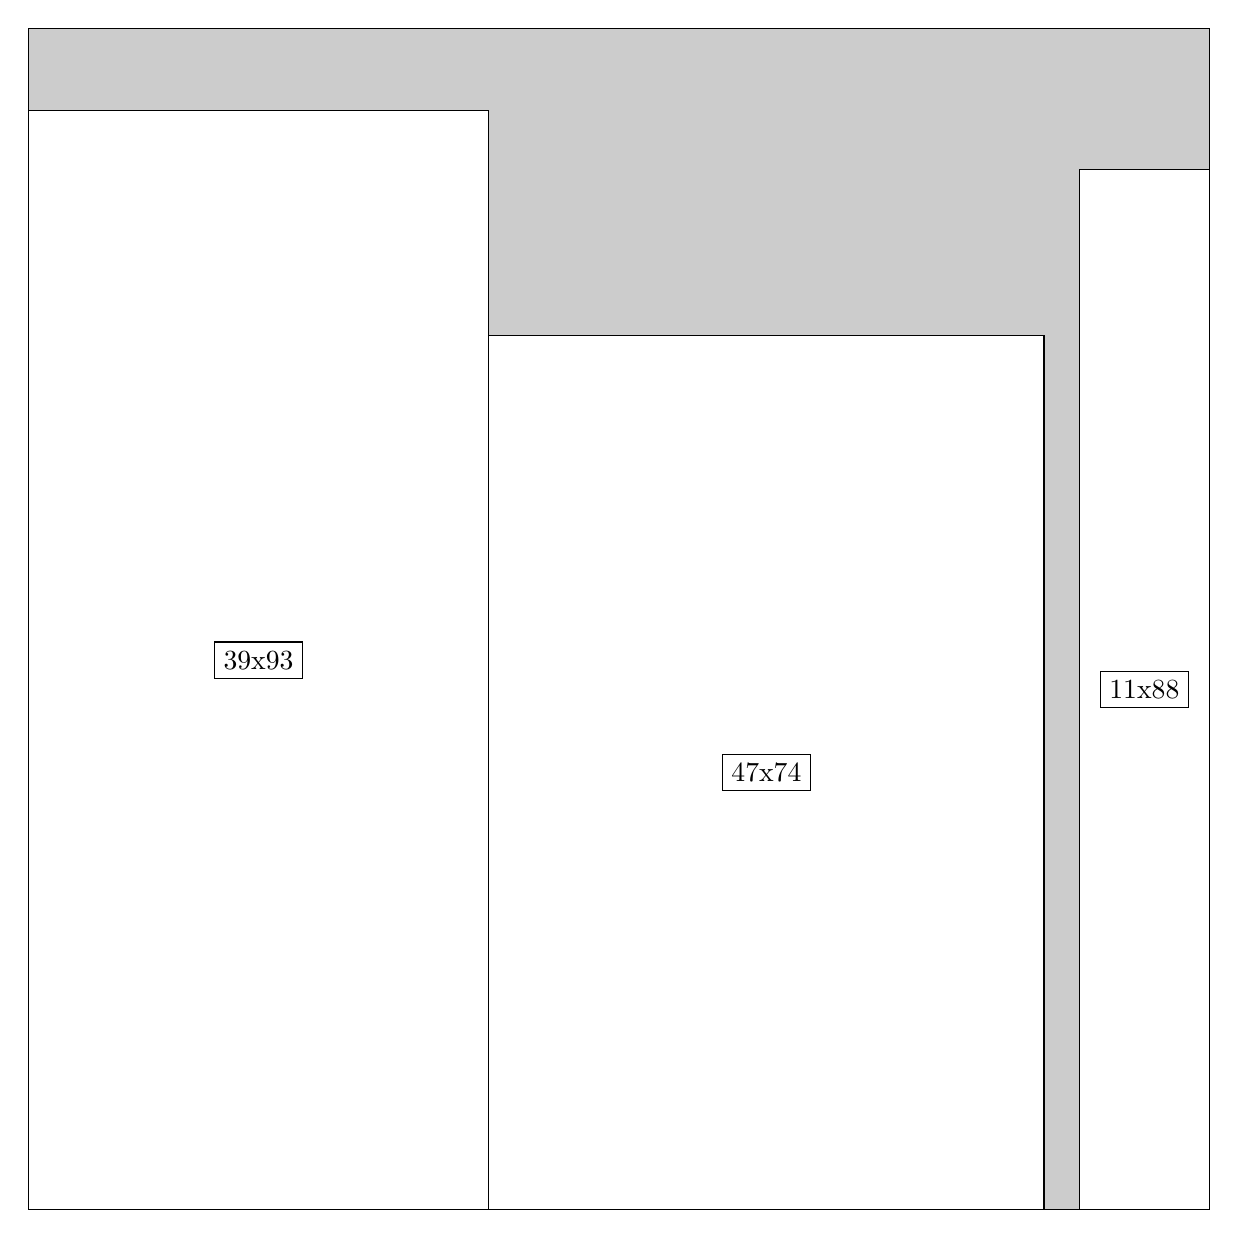
\begin{tikzpicture}[shorten >=1pt,scale=1.0,every node/.style={scale=1.0},->]
\tikzstyle{vertex}=[circle,fill=black!25,minimum size=14pt,inner sep=0pt]
\filldraw[fill=gray!40!white, draw=black] (0,0) rectangle (15.0,15.0);
\foreach \name/\x/\y/\w/\h in {39x93/0.0/0.0/5.85/13.95,47x74/5.85/0.0/7.05/11.1,11x88/13.35/0.0/1.65/13.2}
\filldraw[fill=white!40!white, draw=black] (\x,\y) rectangle node[draw] (\name) {\name} ++(\w,\h);
\end{tikzpicture}


w =39 , h =93 , x =0 , y =0 , v =3627
\par
w =47 , h =74 , x =39 , y =0 , v =3478
\par
w =11 , h =88 , x =89 , y =0 , v =968
\par
\newpage


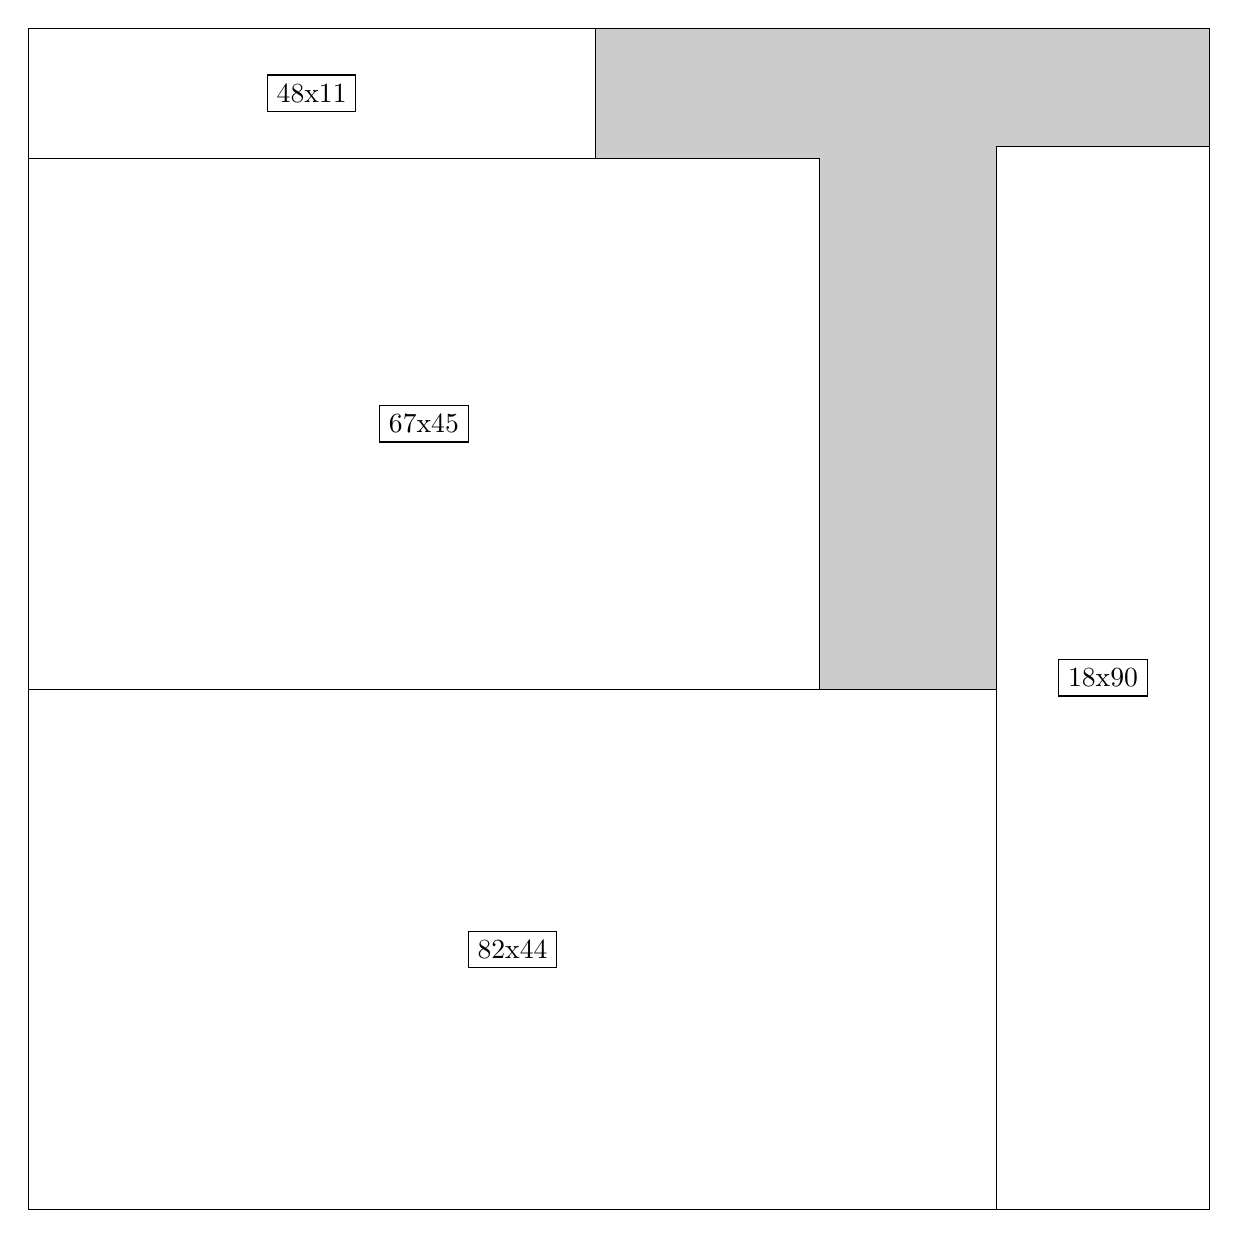
\begin{tikzpicture}[shorten >=1pt,scale=1.0,every node/.style={scale=1.0},->]
\tikzstyle{vertex}=[circle,fill=black!25,minimum size=14pt,inner sep=0pt]
\filldraw[fill=gray!40!white, draw=black] (0,0) rectangle (15.0,15.0);
\foreach \name/\x/\y/\w/\h in {82x44/0.0/0.0/12.299999999999999/6.6,67x45/0.0/6.6/10.049999999999999/6.75,18x90/12.299999999999999/0.0/2.6999999999999997/13.5,48x11/0.0/13.35/7.199999999999999/1.65}
\filldraw[fill=white!40!white, draw=black] (\x,\y) rectangle node[draw] (\name) {\name} ++(\w,\h);
\end{tikzpicture}


w =82 , h =44 , x =0 , y =0 , v =3608
\par
w =67 , h =45 , x =0 , y =44 , v =3015
\par
w =18 , h =90 , x =82 , y =0 , v =1620
\par
w =48 , h =11 , x =0 , y =89 , v =528
\par
\newpage


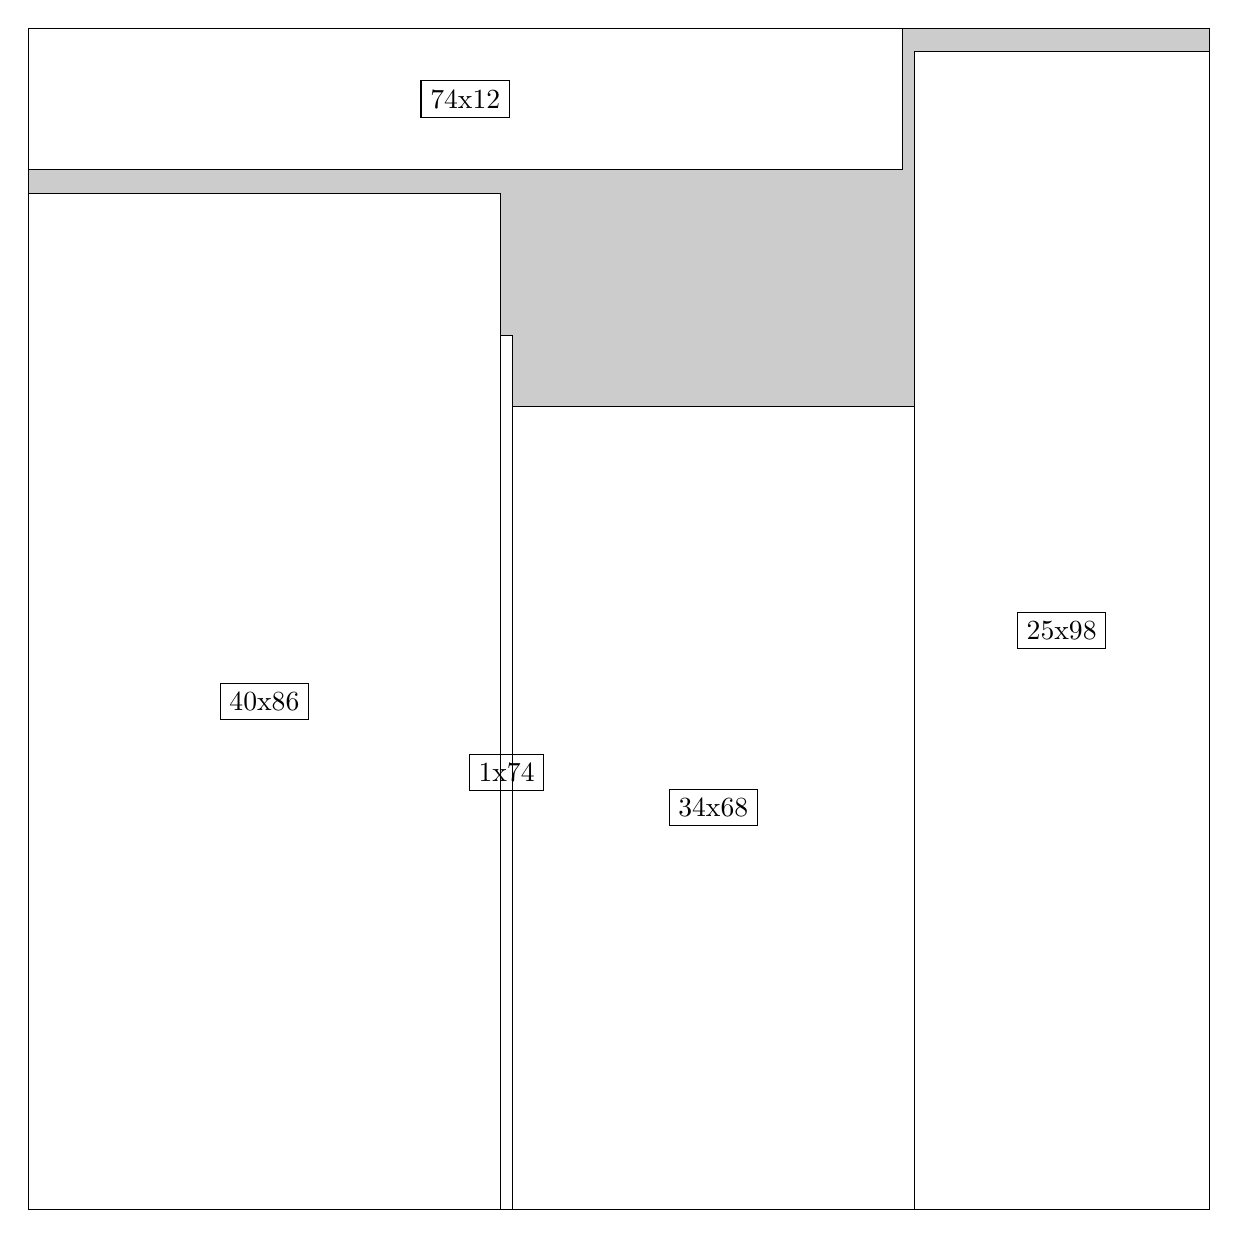
\begin{tikzpicture}[shorten >=1pt,scale=1.0,every node/.style={scale=1.0},->]
\tikzstyle{vertex}=[circle,fill=black!25,minimum size=14pt,inner sep=0pt]
\filldraw[fill=gray!40!white, draw=black] (0,0) rectangle (15.0,15.0);
\foreach \name/\x/\y/\w/\h in {40x86/0.0/0.0/6.0/12.9,25x98/11.25/0.0/3.75/14.7,34x68/6.1499999999999995/0.0/5.1/10.2,74x12/0.0/13.2/11.1/1.7999999999999998,1x74/6.0/0.0/0.15/11.1}
\filldraw[fill=white!40!white, draw=black] (\x,\y) rectangle node[draw] (\name) {\name} ++(\w,\h);
\end{tikzpicture}


w =40 , h =86 , x =0 , y =0 , v =3440
\par
w =25 , h =98 , x =75 , y =0 , v =2450
\par
w =34 , h =68 , x =41 , y =0 , v =2312
\par
w =74 , h =12 , x =0 , y =88 , v =888
\par
w =1 , h =74 , x =40 , y =0 , v =74
\par
\newpage


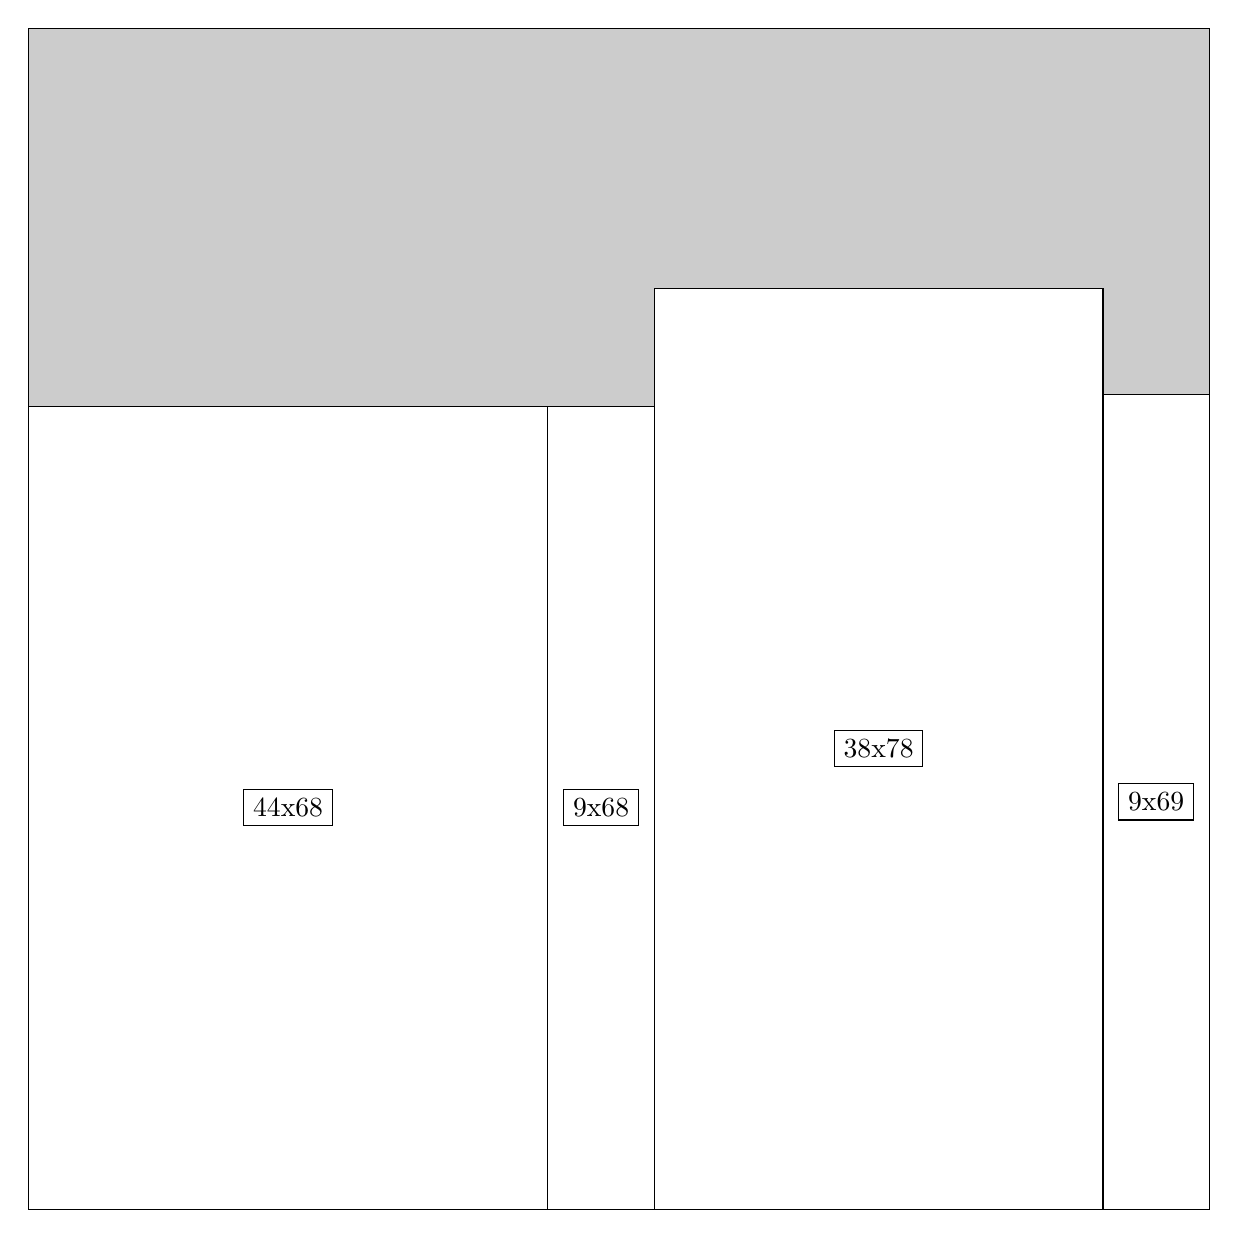
\begin{tikzpicture}[shorten >=1pt,scale=1.0,every node/.style={scale=1.0},->]
\tikzstyle{vertex}=[circle,fill=black!25,minimum size=14pt,inner sep=0pt]
\filldraw[fill=gray!40!white, draw=black] (0,0) rectangle (15.0,15.0);
\foreach \name/\x/\y/\w/\h in {44x68/0.0/0.0/6.6/10.2,38x78/7.949999999999999/0.0/5.7/11.7,9x69/13.65/0.0/1.3499999999999999/10.35,9x68/6.6/0.0/1.3499999999999999/10.2}
\filldraw[fill=white!40!white, draw=black] (\x,\y) rectangle node[draw] (\name) {\name} ++(\w,\h);
\end{tikzpicture}


w =44 , h =68 , x =0 , y =0 , v =2992
\par
w =38 , h =78 , x =53 , y =0 , v =2964
\par
w =9 , h =69 , x =91 , y =0 , v =621
\par
w =9 , h =68 , x =44 , y =0 , v =612
\par
\newpage


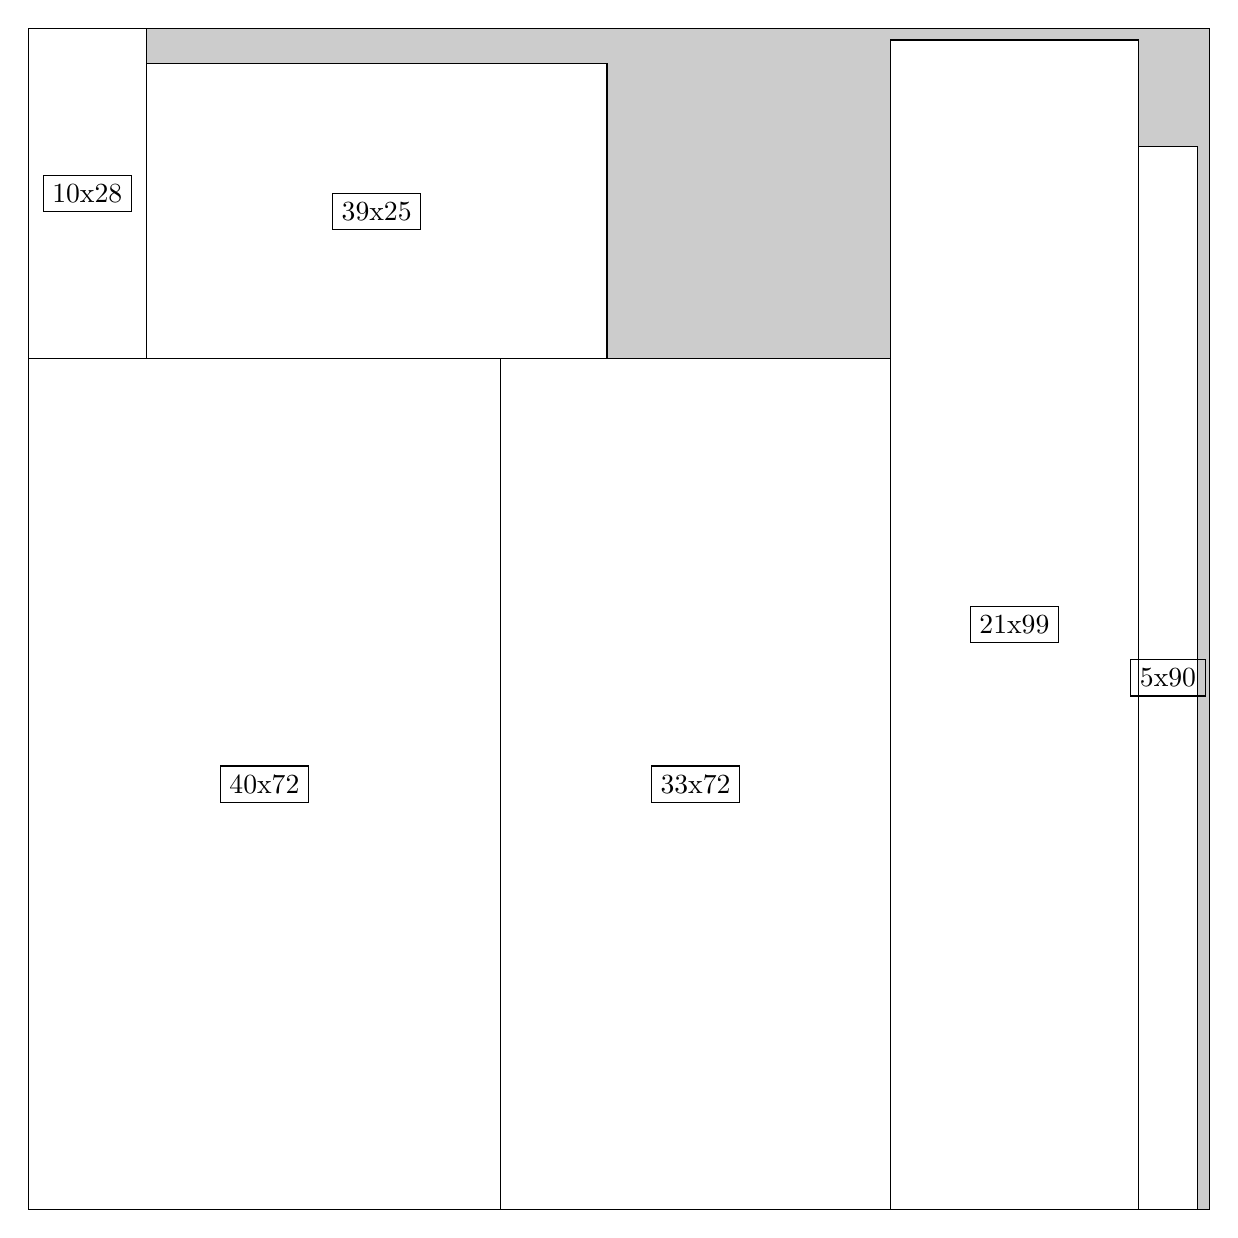
\begin{tikzpicture}[shorten >=1pt,scale=1.0,every node/.style={scale=1.0},->]
\tikzstyle{vertex}=[circle,fill=black!25,minimum size=14pt,inner sep=0pt]
\filldraw[fill=gray!40!white, draw=black] (0,0) rectangle (15.0,15.0);
\foreach \name/\x/\y/\w/\h in {40x72/0.0/0.0/6.0/10.799999999999999,33x72/6.0/0.0/4.95/10.799999999999999,21x99/10.95/0.0/3.15/14.85,39x25/1.5/10.799999999999999/5.85/3.75,5x90/14.1/0.0/0.75/13.5,10x28/0.0/10.799999999999999/1.5/4.2}
\filldraw[fill=white!40!white, draw=black] (\x,\y) rectangle node[draw] (\name) {\name} ++(\w,\h);
\end{tikzpicture}


w =40 , h =72 , x =0 , y =0 , v =2880
\par
w =33 , h =72 , x =40 , y =0 , v =2376
\par
w =21 , h =99 , x =73 , y =0 , v =2079
\par
w =39 , h =25 , x =10 , y =72 , v =975
\par
w =5 , h =90 , x =94 , y =0 , v =450
\par
w =10 , h =28 , x =0 , y =72 , v =280
\par
\newpage


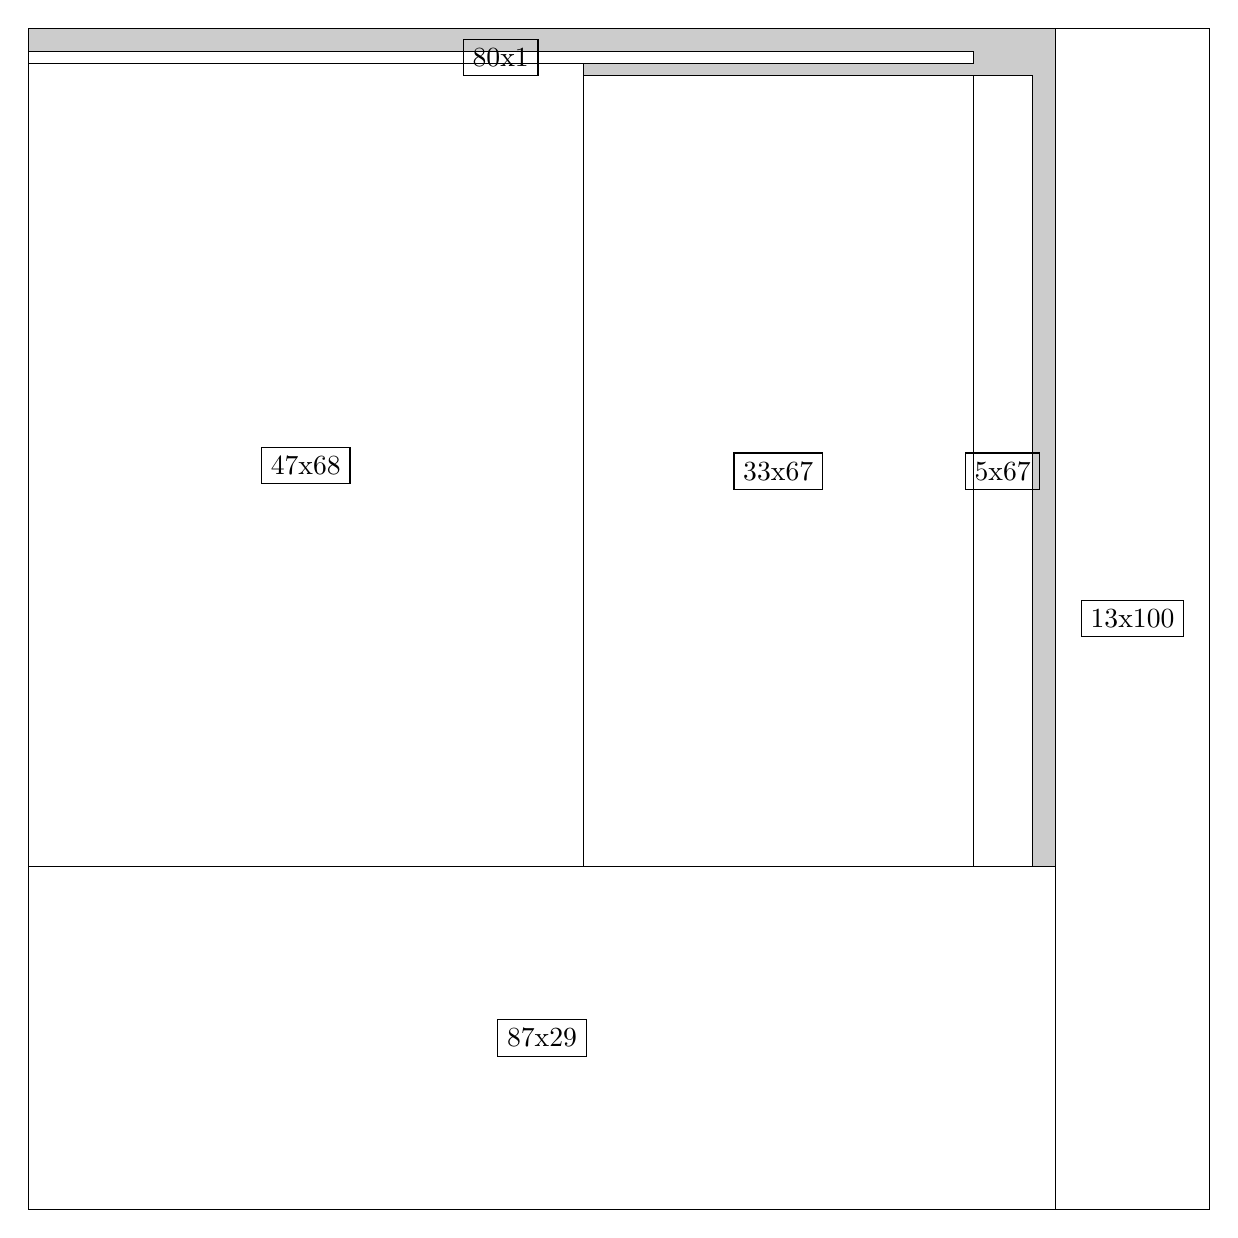
\begin{tikzpicture}[shorten >=1pt,scale=1.0,every node/.style={scale=1.0},->]
\tikzstyle{vertex}=[circle,fill=black!25,minimum size=14pt,inner sep=0pt]
\filldraw[fill=gray!40!white, draw=black] (0,0) rectangle (15.0,15.0);
\foreach \name/\x/\y/\w/\h in {47x68/0.0/4.35/7.05/10.2,33x67/7.05/4.35/4.95/10.049999999999999,87x29/0.0/0.0/13.049999999999999/4.35,13x100/13.049999999999999/0.0/1.95/15.0,5x67/12.0/4.35/0.75/10.049999999999999,80x1/0.0/14.549999999999999/12.0/0.15}
\filldraw[fill=white!40!white, draw=black] (\x,\y) rectangle node[draw] (\name) {\name} ++(\w,\h);
\end{tikzpicture}


w =47 , h =68 , x =0 , y =29 , v =3196
\par
w =33 , h =67 , x =47 , y =29 , v =2211
\par
w =87 , h =29 , x =0 , y =0 , v =2523
\par
w =13 , h =100 , x =87 , y =0 , v =1300
\par
w =5 , h =67 , x =80 , y =29 , v =335
\par
w =80 , h =1 , x =0 , y =97 , v =80
\par
\newpage


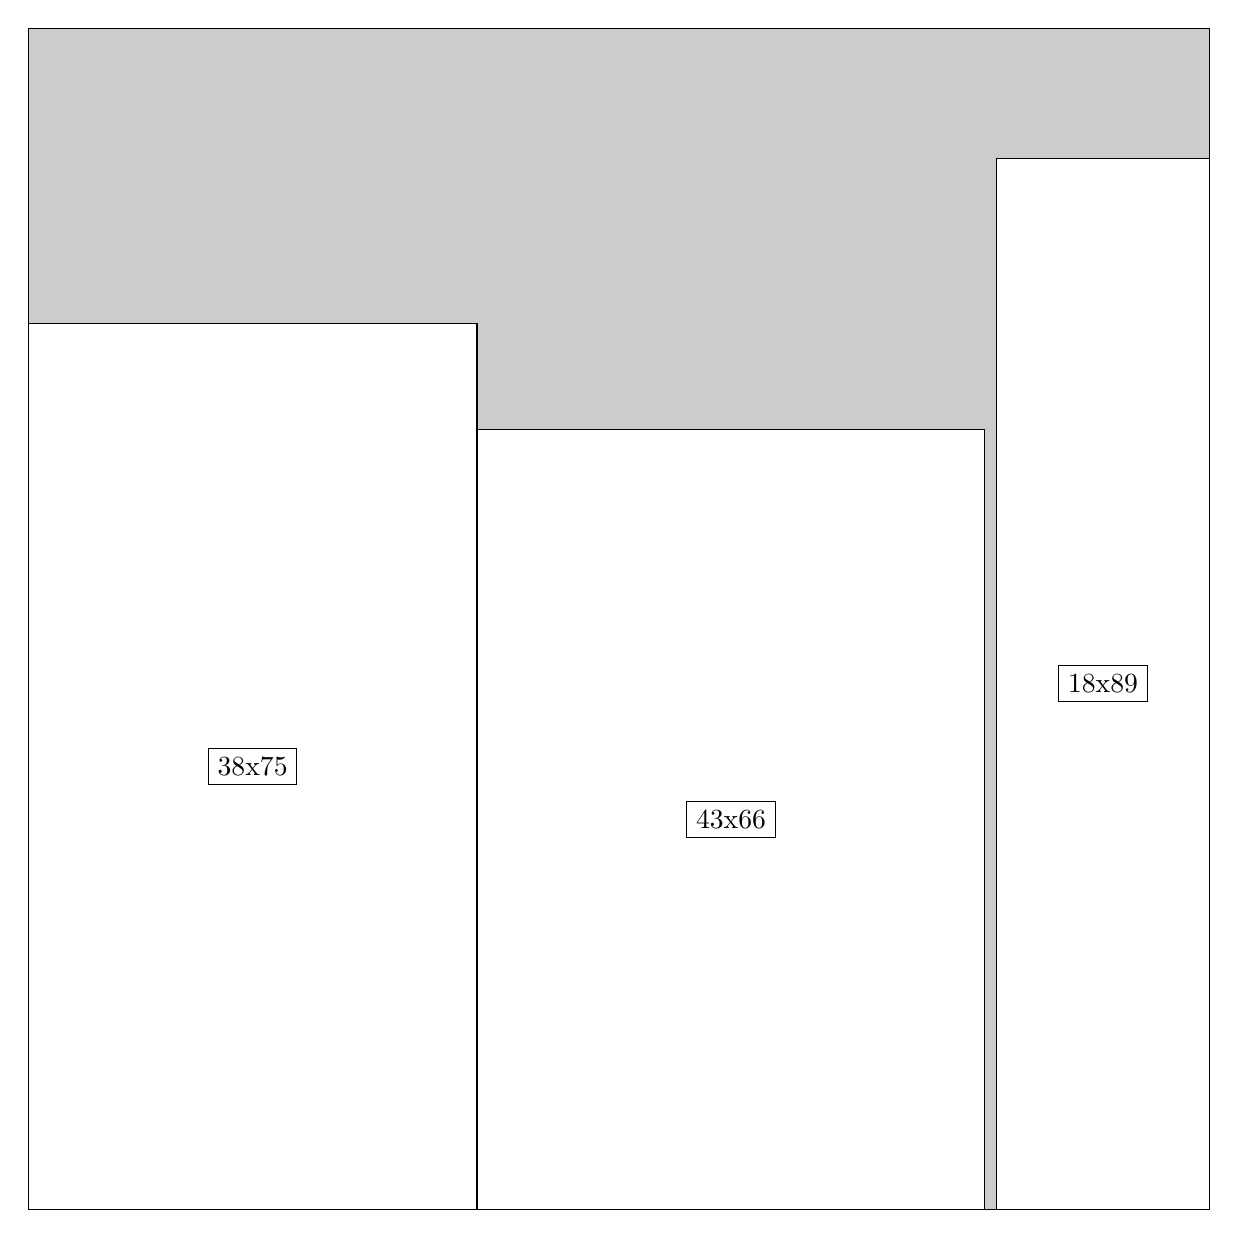
\begin{tikzpicture}[shorten >=1pt,scale=1.0,every node/.style={scale=1.0},->]
\tikzstyle{vertex}=[circle,fill=black!25,minimum size=14pt,inner sep=0pt]
\filldraw[fill=gray!40!white, draw=black] (0,0) rectangle (15.0,15.0);
\foreach \name/\x/\y/\w/\h in {38x75/0.0/0.0/5.7/11.25,43x66/5.7/0.0/6.45/9.9,18x89/12.299999999999999/0.0/2.6999999999999997/13.35}
\filldraw[fill=white!40!white, draw=black] (\x,\y) rectangle node[draw] (\name) {\name} ++(\w,\h);
\end{tikzpicture}


w =38 , h =75 , x =0 , y =0 , v =2850
\par
w =43 , h =66 , x =38 , y =0 , v =2838
\par
w =18 , h =89 , x =82 , y =0 , v =1602
\par
\newpage


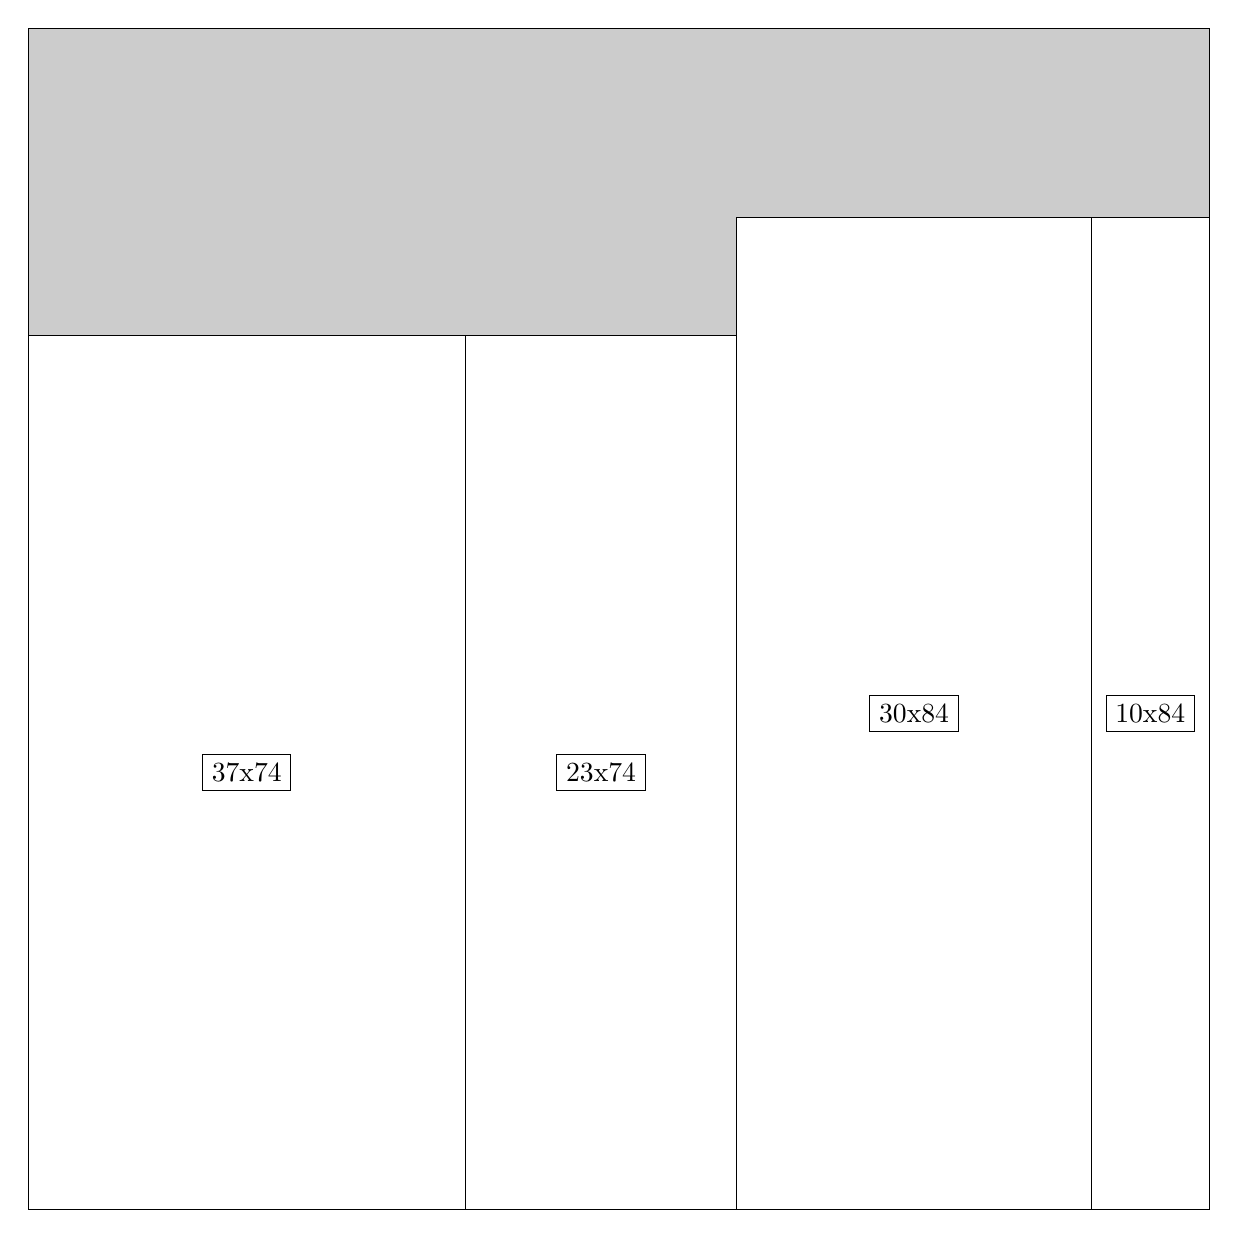
\begin{tikzpicture}[shorten >=1pt,scale=1.0,every node/.style={scale=1.0},->]
\tikzstyle{vertex}=[circle,fill=black!25,minimum size=14pt,inner sep=0pt]
\filldraw[fill=gray!40!white, draw=black] (0,0) rectangle (15.0,15.0);
\foreach \name/\x/\y/\w/\h in {37x74/0.0/0.0/5.55/11.1,30x84/9.0/0.0/4.5/12.6,23x74/5.55/0.0/3.4499999999999997/11.1,10x84/13.5/0.0/1.5/12.6}
\filldraw[fill=white!40!white, draw=black] (\x,\y) rectangle node[draw] (\name) {\name} ++(\w,\h);
\end{tikzpicture}


w =37 , h =74 , x =0 , y =0 , v =2738
\par
w =30 , h =84 , x =60 , y =0 , v =2520
\par
w =23 , h =74 , x =37 , y =0 , v =1702
\par
w =10 , h =84 , x =90 , y =0 , v =840
\par
\newpage


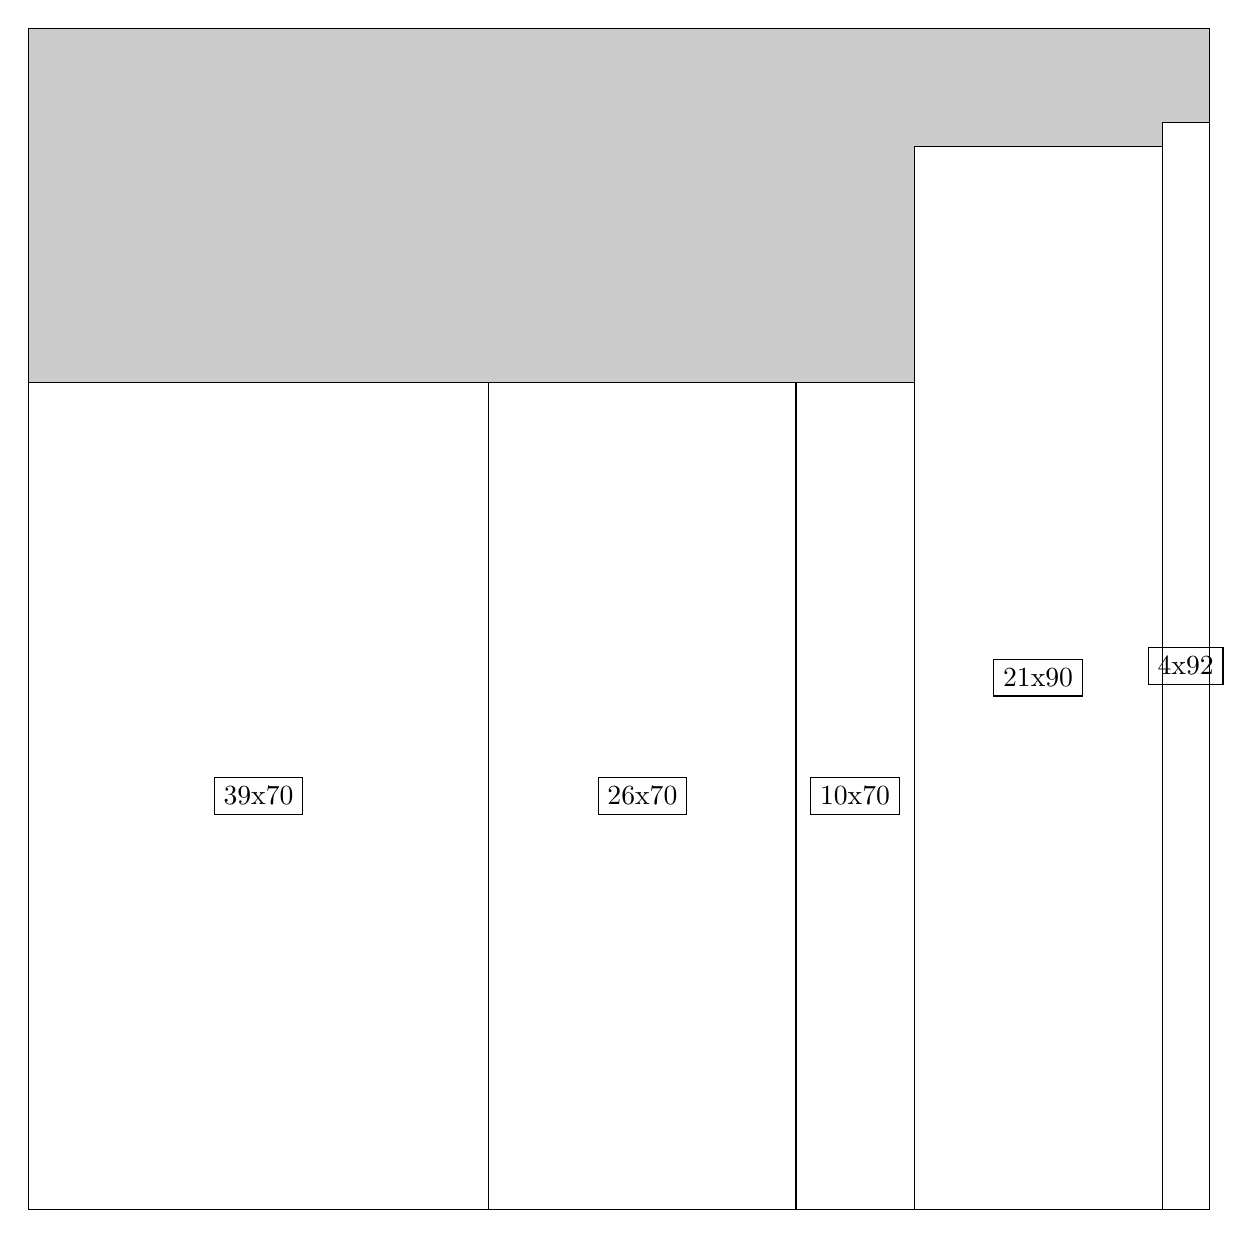
\begin{tikzpicture}[shorten >=1pt,scale=1.0,every node/.style={scale=1.0},->]
\tikzstyle{vertex}=[circle,fill=black!25,minimum size=14pt,inner sep=0pt]
\filldraw[fill=gray!40!white, draw=black] (0,0) rectangle (15.0,15.0);
\foreach \name/\x/\y/\w/\h in {39x70/0.0/0.0/5.85/10.5,21x90/11.25/0.0/3.15/13.5,26x70/5.85/0.0/3.9/10.5,10x70/9.75/0.0/1.5/10.5,4x92/14.399999999999999/0.0/0.6/13.799999999999999}
\filldraw[fill=white!40!white, draw=black] (\x,\y) rectangle node[draw] (\name) {\name} ++(\w,\h);
\end{tikzpicture}


w =39 , h =70 , x =0 , y =0 , v =2730
\par
w =21 , h =90 , x =75 , y =0 , v =1890
\par
w =26 , h =70 , x =39 , y =0 , v =1820
\par
w =10 , h =70 , x =65 , y =0 , v =700
\par
w =4 , h =92 , x =96 , y =0 , v =368
\par
\newpage


\end{document}